\documentclass[twocolumn=on,fontsize=12pt,DIV=calc]{scrartcl}
\usepackage[portuguese]{babel}
\usepackage[utf8]{inputenc}
\usepackage[hidelinks]{hyperref}
\usepackage{amsmath,amsfonts,amsthm}
\usepackage[varg]{txfonts}
\usepackage{microtype}
\usepackage{graphicx}

\newcommand{\dpar}[1]{\left(#1\right)}
\newcommand{\dsqr}[1]{\left[#1\right]}

% \newtheoremstyle{example}{}{}{}{}{}{.}{ }{}
% \theoremstyle{example}
\theoremstyle{definition}
\newtheorem{ex}{Exercício}[section]

\DeclareMathOperator{\sen}{sen}

\title{Notas de Física Geral 2}

\author{Max Jáuregui}

\begin{document}
\maketitle
\tableofcontents

\section{Equilíbrio de um corpo rí\-gi\-do}

Considere uma partícula de massa $m$ na posição $\vec r$ sobre a qual
atua uma força $\vec F$. O \textbf{torque} da força $\vec F$ é definido
por $\vec\tau=\vec r\times\vec F$, onde $\times$ denota o
\textbf{produto vetorial} de dois vetores, o qual é definido por
\begin{equation*}
  \begin{split}
    \vec A\times\vec B&= \left|
      \begin{array}{ccc}
        \hat i&\hat j&\hat k\\
        A_x&A_y&A_z\\
        B_x&B_y&B_z
      \end{array}
    \right|\\
    &=(A_yB_z-A_zB_y)\hat i+(A_zB_x-A_xB_z)\hat j\\
    &\quad+(A_xB_y-A_yB_x)\hat k\,.
  \end{split}
\end{equation*}
A unidade do torque no sistema internacional (SI) é
$\mathrm{N}\cdot\mathrm{m}$.

\begin{ex}
  Verifique que, para uma par\-tí\-cu\-la de $10\,\mathrm{kg}$ na posição
  $\vec r=\cos 30^\circ\hat i+\sen 30^\circ\hat j$ (em metros), o
  torque do peso é igual a $-49\sqrt{3}\hat k$ (em
  $\mathrm{N}\cdot \mathrm{m}$).
\end{ex}

Usaremos a notação $\dot{\vec a}$ para representar a derivada de
$\vec a$ em relação ao tempo, ou seja,
$\dot{\vec a}=\frac{d\vec a}{dt}$.

\begin{ex}
  Considere uma partícula de massa $m$ na posição $\vec r$ sobre a
  qual atua uma força $\vec F$. Definindo o \textbf{momento angular} de
  uma partícula por
  $$\vec L=\vec r\times\vec p\,,$$
   onde $\vec p$ é o  momento linear da partícula, mostre que $\vec\tau=\dot{\vec
    L}$. Isso quer dizer que o torque da força $\vec F$ é igual à taxa
  de variação do momento angular da partícula (note a semelhança com a
  segunda lei de Newton). A unidade de momento angular no SI é
  $\mathrm{kg}\cdot\mathrm{m^2/s}$.

  \noindent\textit{Dica:} Na expressão do torque substitua $\vec F$ por
  $\dot{\vec p}$, em virtude da segunda lei de Newton
  ($\vec F=\dot{\vec p}$). Logo, utilize a identidade
  $\frac{d}{dt}(\vec r\times\vec p)=\dot{\vec r}\times\vec p+\vec
  r\times\dot{\vec p}$ e use o fato de que
  $\dot{\vec r}\times\vec p=0$, pois o vetor velocidade $\dot{\vec r}$
  é paralelo a $\vec p$.
\end{ex}

\begin{ex}
  Considere duas partículas de massas $m_1$ e $m_2$ sobre as quais
  atuam forças externas $\vec F_1$ e $\vec F_2$ respectivamente. Além
  das forças externas, há forças internas $\vec F_{12}$ (sobre a
  partícula $1$) e $\vec F_{21}$ (sobre a partícula $2$) devido a
  interação das partículas (por exemplo, interação gravitacional ou
  elétrica), as quais são paralelas ao vetor $\vec r_1-\vec
  r_2$. Mostre que
  \begin{equation}
    \label{eq:1}
    \vec F_1+\vec F_2=\dot{\vec p}_1+\dot{\vec p}_2\quad\text{e}\quad\vec\tau_1+\vec\tau_2=\dot{\vec L}_1+\dot{\vec L}_2\,.
  \end{equation}

  \noindent\textit{Dica:} Segue da segunda lei de Newton que
  \begin{equation}
    \label{eq:2}
      \vec F_1+\vec F_{12}=\dot{\vec p}_1\quad\text{e}\quad\vec F_2+\vec F_{21}=\dot{\vec p}_2\,.
  \end{equation}
  Somando essas equações e usando a terceira lei de Newton
  ($\vec F_{12}=-\vec F_{21}$), obtém-se a primeira equação
  em~(\ref{eq:1}). Para se obter a segunda equação em~(\ref{eq:1}),
  multiplicam-se vetorialmente à esquerda as equações~(\ref{eq:2})
  pelos vetores posição $\vec r_1$ e $\vec r_2$ respectivamente. Logo,
  somam-se as equações obtidas e usa-se o fato de que
  $(\vec r_1-\vec r_2)\times\vec F_{12}=\vec 0$.
\end{ex}

O exemplo anterior pode ser generalizado sem realizar nenhuma
alteração fundamental para o caso de um sistema de $n$
partículas. Nesse caso vamos ter que
\begin{equation}
  \label{eq:3}
    \vec F_{\mathrm{ext}}=\dot{\vec p}\quad\text{e}\quad
    \vec \tau_{\mathrm{ext}}=\dot{\vec L}\,,
\end{equation}
onde $\vec F_{\mathrm{ext}}=\vec F_1+\cdots+\vec F_n$ é a força
externa total sobre o sistema, $\vec p=\vec p_1+\cdots+\vec p_n$ é o
momento linear total do sistema,
$\vec\tau_{\mathrm{ext}}=\vec\tau_1+\cdots+\vec\tau_n$ é o torque
externo total sobre o sistema e $\vec L=\vec L_1+\cdots+\vec L_n$ é o
momento angular total do sistema.

Um \textbf{corpo rígido} é um corpo não pontual que não se deforma. O
fato de um corpo rígido não se deformar equivale a dizer que a
distância entre dois pontos quaisquer do corpo é uma constante.

Para estudar a dinâmica de um corpo rígido, podemos dividir ele em $n$
partes pequenas e assim considerar o corpo rígido como um sistema de
$n$ corpos. Se a massa da $i$-ésima parte é $\Delta m_i$, sua posição
é $\vec r_i$ e sua velocidade é $\vec v_i$, então o momentum total do
sistema é
$$\vec p=\sum_{i=1}^n\vec v_i\Delta m_i$$
e o momento angular total do sistema é
$$\vec L=\sum_{i=1}^n(\vec r_i\times\vec v_i)\Delta m_i\,.$$
Considerando que o número de partes $n$ tende ao infinito e
simultaneamente a massa de cada parte tende a zero, as somas
anteriores tornam-se integrais. Dessa maneira, encontramos que o
\textbf{momento linear do corpo rígido} é dado por
\begin{equation}
  \label{eq:4}
  \vec p=\int \vec v\,dm
\end{equation}
e o \textbf{momento angular do corpo rígido} por
\begin{equation}
  \label{eq:5}
  \vec L=\int (\vec r\times\vec v)\,dm\,,
\end{equation}
onde as integrais são sobre toda a massa do corpo rígido.

As Eqs.~(\ref{eq:3}) continuam valendo da mesma forma para um corpo
rígido, levando em conta que $\vec p$ e $\vec L$ são dadas pelas
Eqs.~(\ref{eq:4}) e~(\ref{eq:5}).

O movimento de um corpo rígido pode ser estudado analisando
separadamente os movimentos de translação e de rotação em torno de um
eixo que passa pelo corpo.

\begin{ex}
  Considere um corpo rígido de massa $M$ que realiza um movimento de
  translação pura com velocidade $\vec v$. Mostre que nesse caso
  $$\vec p=M\vec v\quad\text{e}\quad\vec L=\vec R\times\vec p\,,$$
  onde
  $$\vec R=\frac{1}{M}\int \vec r\,dm$$
  é a posição do \textbf{centro de massa} do corpo.

  \noindent\textit{Dica:} Quando um corpo rígido realiza um movimento de translação pura, todos os pontos do corpo possuem a mesma velocidade. Dessa forma, a
  velocidade $\vec v$ pode sair das integrais nas Eqs.~(\ref{eq:4})
  e~(\ref{eq:5}).
\end{ex}

O exercício anterior nos diz que um corpo rígido que realiza um
movimento de translação pura se comporta como uma partícula de massa
$M$ localizada no centro de massa do corpo. Em outras palavras, as
dimensões do corpo rígido não são relevantes no movimento de
translação.

Diferentemente do caso do movimento de trans\-la\-ção, quando um corpo
rígido realiza um movimento de rotação ao redor de um eixo que passa
por ele, os pontos do corpo que estão mais próximos do eixo de rotação
tem velocidade menor do que os pontos mais afastados. Logo, nesse caso
a velocidade $\vec v$ não pode sair da integral nas Eqs.~(\ref{eq:4})
e~(\ref{eq:5}).

Para simplificar nosso estudo do movimento de rotação de um corpo
rígido, vamos considerar um corpo homogêneo (massa distribuída
uniformemente) e simétrico. Além disso, vamos analisar o caso em que o
corpo gira em torno de um dos seus eixos de simetria com velocidade
angular $\vec\omega$.

Antes de continuar, lembramos que, para uma partícula que realiza um
movimento circular com velocidade angular $\vec\omega$, vale a relação
vetorial $\vec v=\vec\omega\times\vec r$, onde $\vec v$ é a velocidade
da partícula e $\vec r$ é sua posição em relação a um sistema de
referência fixo ao eixo de rotação.

Continuando nossa análise da rotação de um corpo rígido, vemos que o
momento angular do corpo é dado por
$$\vec L=\int [\vec r\times(\vec\omega\times\vec r)]\,dm\,,$$
onde a posição $\vec r$ é em relação a um sistema de referência fixo
ao eixo de rotação.  Usando a identidade vetorial
$$\vec a\times(\vec b\times\vec c)=(\vec a\cdot\vec c)\vec b-(\vec a\cdot\vec b)\vec c\,,$$
temos que
\begin{equation}
  \label{eq:6}
  \vec L=\int [(\vec r\cdot\vec r)\vec\omega-(\vec r\cdot\vec\omega)\vec r]\,dm\,.
\end{equation}
Se $\theta$ é o ângulo entre os vetores $\vec\omega$ e $\vec r$, então
$\vec r\cdot\vec \omega=r\omega\cos\theta$ e, por conseguinte,
$$\vec L=\int [r^2\vec\omega-(r\omega\cos\theta)\vec r]\,dm\,.$$
Devido a que o corpo gira em torno de um eixo de simetria, podemos
inferir que o vetor $\vec L$ deve ter a mesma direção que o vetor
$\vec\omega$. Isso quer dizer que as direções perpendiculares a
$\vec\omega$ devem se anular após fazer a integral na
Eq.~(\ref{eq:6}). Logo, vamos ter
\begin{equation*}
  \begin{split}
    \vec L&=\int \dpar{r^2\vec\omega-(r\omega\cos\theta)(r\cos\theta)\frac{\vec\omega}{\omega}}\,dm\\
    &=\int (r^2-r^2\cos^2\theta)\vec\omega\,dm\\
    &=\int (r^2\sen^2\theta)\vec\omega\,dm\,.
  \end{split}
\end{equation*}
Como todo ponto do corpo rígido gira com a mesma velocidade angular,
obtemos que
\begin{equation}
  \label{eq:7}
  \vec L=I\vec\omega\,,
\end{equation}
onde
\begin{equation}
  \label{eq:8}
  I=\int (r\sen\theta)^2\,dm
\end{equation}
é o chamado \textbf{momento de inércia} do corpo. Cabe ressaltar que
para cada ponto do corpo, $r\sen\theta$ é a distância do ponto ao eixo
de rotação.

A Eq.~(\ref{eq:7}) nos diz que o momento angular é um indicador da
rotação de um corpo rígido.

Um corpo rígido está em \textbf{equi\-lí\-brio es\-tá\-ti\-co} quando não realiza
movimento de translação nem de rotação.

Se um corpo rígido está em equilíbrio estático, todo ponto do corpo
tem velocidade nula. Logo, segue das Eqs.~(\ref{eq:4}) e~(\ref{eq:5})
que nesse caso vamos ter $\vec p=\vec 0$ e $\vec L=\vec 0$,
onde, na segunda condição, $\vec L$ pode ser calculado em relação a
qualquer ponto. Substituindo isso nas Eqs.~(\ref{eq:3}), obtemos as
chamadas \textbf{condições de equilíbrio} para o corpo rígido:
\begin{equation}
  \label{eq:9}
  {\vec F}_{\mathrm{ext}}=\vec 0\quad\text{e}\quad \vec\tau_{\mathrm{ext}}=\vec 0\,,
\end{equation}
onde, na segunda condição, $\vec\tau_{\mathrm{ext}}$ pode ser
calculado em relação a qualquer ponto.

O fato de um corpo rígido satisfazer uma das condições dadas na
Eq.~(\ref{eq:9}) não implica que a outra será também satisfeita. Por
exemplo, se temos uma barra sobre uma mesa e aplicamos forças de
direções opostas sobre os extremos da barra e perpendiculares a ela, a
primeira condição em~(\ref{eq:9}) é satisfeita, mas a segunda não.

\begin{ex}
  \label{ex:1}
  Considere um corpo rígido de massa $M$. Se a aceleração da gravidade
  $\vec g$ é constante, mostre que o torque do peso do corpo é dado
  por
  $$\vec\tau_P=\vec R\times(M\vec g)\,,$$
  onde $\vec R$ é a posição do
  centro de massa do corpo. Em outras palavras, o torque do peso do
  corpo rígido pode ser calculado considerando o corpo como uma
  partícula de massa $M$ localizada no centro de massa do corpo.

  \noindent\textit{Dica:} O torque do peso de um corpo rígido é igual
  à soma de todos os torques dos pesos das partes do corpo. Quando o
  número de partes tende a infinito e a massa de cada parte tende a
  zero, essa soma torna-se uma integral. Dessa forma,
  $\vec\tau_P=\int (\vec r\times\vec g)\,dm$.
\end{ex}

Define-se o \textbf{centro de gravidade} de um corpo rígido de massa $M$
como o ponto no qual uma partícula de massa $M$ teria um torque do
peso igual ao torque do peso do corpo rígido. O exercício anterior
mostra que, se $\vec g$ é constante (por exemplo, na superfície da
Terra), o centro de gravidade de um corpo rígido coincide com seu
centro de massa. Para nossos fins, centro de gravidade e centro de
massa serão equivalentes.

Se um corpo rígido é homogêneo e tem um eixo de simetria, o centro de
massa do corpo estará localizado em algum ponto desse eixo.

Se um corpo rígido é pendurado a partir de um ponto arbitrário e está
em equilíbrio, o centro de massa do corpo deve estar localizado em
algum ponto da linha vertical que passa pelo ponto de suspensão. Com
efeito, como nesse caso o torque do peso deve ser nulo, segue do
exercício~\ref{ex:1} que $\vec R$ e $\vec g$ devem ser vetores
paralelos, ou seja, $\vec R$ deve ser um vetor vertical.

Se consideramos uma pessoa como um corpo rígido, quando a pessoa se
equilibra em um pé só, o centro de massa dela deve estar na linha
vertical que passa pelo pé de suporte. Para isso é necessário realizar
um deslocamento do centro de massa, o qual pode não ser possível se a
pessoa está junto a uma parede.

\begin{ex}
  Considere um corpo rígido em um plano inclinado de superfície
  rugosa, como ilustrado na figura~\ref{fig:tombo}A. Dê argumentos que
  indiquem que o corpo pode de fato estar em equilíbrio (não vai
  tombar).

  \noindent\textit{Dica:} Desenhe as forças que atuam sobre o
  corpo. As forças normais e de atrito podem assumir valores de tal
  forma que a força resultante sobre o corpo seja nula. Para calcular
  os torques das forças escolha o ponto de apoio mais baixo, pois, em
  relação a esse ponto, os torques das forças de atrito e da normal
  que atua nesse ponto são nulos. Logo, mostre que o torque externo
  total pode ser escrito como
  $\vec \tau_{\mathrm{ext}}=\vec\tau_P+\vec\tau_N$, onde $\vec\tau_P$
  e $\vec\tau_N$ têm direções opostas.
  \begin{figure}[ht]
    \centering
    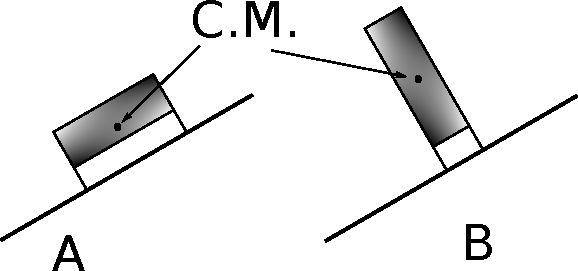
\includegraphics[width=0.45\textwidth,keepaspectratio]{aux/tombo.pdf}
    \caption{Estudo do tombo de um corpo rígido.}
    \label{fig:tombo}
  \end{figure}
\end{ex}

\begin{ex}
  Considere um corpo rígido em um plano inclinado de superfície
  rugosa, como ilustrado na figura~\ref{fig:tombo}B. Dê argumentos que
  indiquem que o corpo não pode estar em equilíbrio (vai tombar).

  \noindent\textit{Dica:} Proceda da mesma forma que no exercício
  anterior. Mostre que o torque externo total pode ser escrito como
  $\vec\tau_{\mathrm{ext}}=\vec\tau_P+\vec\tau_N$, onde $\vec\tau_P$ e
  $\vec\tau_N$ têm a mesma direção.
\end{ex}

Suponhamos que queremos calcular o torque de uma força $\vec F$
aplicada sobre um ponto de um corpo rígido que se encontra na posição
$\vec r$ em relação a um ponto arbitrário $O$. Por definição esse
torque estará dado por $\vec\tau=\vec r\times\vec F$. Porém, às vezes
o módulo de $\vec r$ ou sua direção podem ser difíceis de se
conhecer. Para dar conta desse problema, observamos que se $\vec r'$ é
um vetor qualquer paralelo a $\vec F$, então $\vec r'\times\vec F=0$
e, por conseguinte, $\vec\tau=(\vec r+\vec r')\times \vec F$. Dessa
maneira, escolhendo o vetor $\vec r'$ de forma conveniente podemos
calcular $\vec\tau$ de forma mais simples. Em particular, se
$\vec r+\vec r'$ é um vetor perpendicular a $\vec F$, então
$\tau=|\vec r+\vec r'|F$.

Na maioria dos exercícios lidaremos com problemas onde as posições e
as forças se encontram em um plano; especificamente, o plano do
papel. Dessa forma, os torques das forças sempre serão vetores
perpendiculares ao papel. Devido a isso, podemos adotar a seguinte
convenção: se o vetor torque aponta para fora do papel, consideraremos
ele como positivo; caso contrário, consideraremos ele como
negativo. Uma regra prática para determinar o sinal do torque de uma
força é a seguinte: se a força tende a fazer girar o corpo em sentido
antihorário em relação ao ponto de referência, o torque será positivo;
caso contrário, será negativo.

\begin{ex}
  Uma barra homogênea de $12\,\mathrm{kg}$ está em equilíbrio
  estático. Um extremo dela está apoiada em uma parede rugosa e o
  outro está amarrado a uma corda como ilustrado na
  figura~\ref{fig:barra_equilibrio}. (i) Encontre o valor da tensão na
  corda. (ii) Encontre o valor da força de atrito sobre a barra devido
  à parede.

  \noindent\textit{Dica:} Considere o ponto de apoio da barra na parede como o ponto de referência para o cálculo de torques. Com isso, encontre o valor da tensão na corda.
  \begin{figure}[ht]
    \centering
    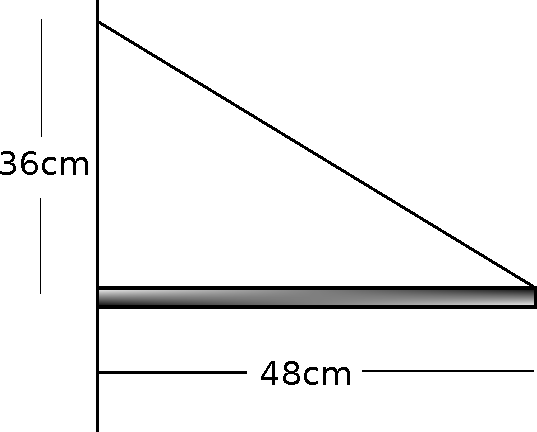
\includegraphics[width=0.45\textwidth,keepaspectratio]{aux/barra_equilibrio.pdf}
    \caption{Barra homogênea em equilíbrio es\-tá\-ti\-co.}
    \label{fig:barra_equilibrio}
  \end{figure}
\end{ex}

\begin{ex}
  Uma escada homogênea de $8\,\mathrm{m}$ de comprimento e
  $5\,\mathrm{kg}$ de massa é apoiada em uma parede vertical lisa
  fazendo um ângulo de $60^\circ$ com o chão. Se uma pessoa de
  $70\,\mathrm{kg}$ está sobre a escada e ela se encontra em
  equilíbrio estático, determine o valor da força de atrito sobre a
  base da escada quando a pessoa andou na escada (i) $4\,\mathrm{m}$ e
  (ii) $6\,\mathrm{m}$.

  \noindent\textit{Dica:} Usando a condição de equilíbrio $\vec F_{\textrm{ext}}=\vec 0$, obtenha
  que o valor da força de atrito é igual à força normal devido à
  parede. Use a condição $\vec\tau_\textrm{ext}=\vec 0$ para encontrar o
  valor dessa força normal, tomando como ponto de referência para o
  cálculo de torques o ponto mais baixo da escada.
\end{ex}

\begin{ex}
  Uma roda homogênea de massa $M$ e raio $R$ se encontra atascada
  devido a um desnível do chão. Qual deve ser o valor mínimo de uma
  força $\vec F$ horizontal aplicada no centro de massa da roda para
  que a ela comece a se mover? Esse valor mínimo é menor se a força é
  aplicada no ponto mais alto da roda?

  \noindent\textit{Dica:} Se a bola está prestes a se mover, a força
  normal devido ao chão é nula. Use a condição de equilíbrio
  $\vec\tau_{\mathrm{ext}}=0$ considerando o ponto mais alto do
  desnível como ponto de referência para o cálculo de torques.
  \begin{figure}[ht]
    \centering
    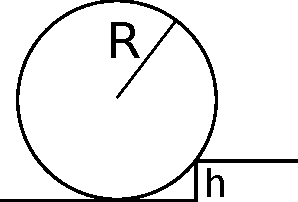
\includegraphics[width=0.45\textwidth,keepaspectratio]{aux/roda_obstaculo.pdf}
    \caption{Roda atascada devido a um desnível do chão.}
    \label{fig:roda_obstaculo}
  \end{figure}
\end{ex}

\begin{ex}
  Quando temos um bloco homogêneo na borda de uma mesa e queremos que
  ele esteja em equilíbrio estático, o centro de massa do bloco deve
  se encontrar dentro da mesa. Considere agora dois blocos homogêneos
  de comprimento $l$. (i) Determine as condições para que ao se
  colocar um bloco sobre o outro na borda da mesa eles estejam em
  equilíbrio estático. (ii) Determine a distância máxima entre o
  extremo da mesa ao extremo do bloco superior.

  \noindent\textit{Dica:} Se $x_1$ e $x_2$ são as posições horizontais
  dos centros de massa dos blocos em relação ao bordo da mesa
  (origem), deve-se ter $x_1\le 0$, $x_2\le l/2+x_1$ e $x_1+x_2\le
  0$. Para maximizar a distância entre o extremo da mesa e o extremo
  do bloco $2$, nas condições anteriores devemos considerar
  $x_2=l/2+x_1$ e $x_1+x_2=0$.
\end{ex}

\begin{ex}
  No espírito do exercício anterior, considere agora três blocos
  homogêneos de comprimento $l$ e determine a distância máxima entre o
  extremo da mesa ao extremo do bloco superior. Generalizando seu
  resultado, infira que ao empilhar $n$ blocos, a distância máxima
  entre o extremo da mesa e o extremo do bloco superior é dada por
  $$d=\frac{l}{2}\dpar{1+\frac{1}{2}+\frac{1}{3}+\cdots+\frac{1}{n}}\,.$$
  Mostre que usando $4$ blocos vamos ter $d>l$.

  \noindent\textit{Dica:} Primeiramente considere os dois blocos de
  cima como um bloco só e encontre as posições dos centros de massa
  desse bloco grande e do bloco de baixo. Logo, use o resultado do
  exercício anterior para colocar os dois blocos de cima de tal forma
  que $d$ tenha o maior valor possível.
\end{ex}

\section{Gravitação newtoniana}

Estudando o movimento da Lua e dos planetas, Newton concluiu que
existe uma força atrativa entre dois corpos quaisquer, chamada de
\textbf{força gravitacional}. Mais precisamente, ele encontrou a
seguinte expressão para o valor da força gravitacional entre duas
partículas de massas $m_1$ e $m_2$ separadas por uma distância $r$:
$$F_g=\frac{Gm_1m_2}{r^2}\,,$$
onde $G$ é uma constante chamada de \textbf{constante gravitacional}.
Sobre cada partícula atua uma força de módulo $F_g$ que aponta na
direção da outra partícula, ou seja, as partículas se atraem. Dessa
maneira, se as partículas estão nas posições $\vec r_1$ e $\vec r_2$,
a força gravitacional sobre a partícula $1$ devido à partícula $2$ é
dada vetorialmente por
$$\vec F_{12}=\frac{Gm_1m_2}{|\vec r_1-\vec r_2|^3}(\vec r_2-\vec r_1)$$
e a força sobre a partícula $2$ devido à partícula $1$ é
$$\vec F_{21}=\frac{Gm_1m_2}{|\vec r_1-\vec r_2|^3}(\vec r_1-\vec r_2)\,.$$

O valor da constante gravitacional $G$ pode ser encontrado
experimentalmente. Quase 100 anos depois de Newton publicar sua lei da
gravitação (junto com as três leis de Newton), Cavendish conseguiu
medir o valor de $G$ usando uma balança de torção (ver livro). O valor
que ele encontrou estava próximo do valor atualmente aceito, que é
$$G=6{,}67\times 10^{-11}\,\mathrm{N}\cdot\mathrm{m}^2/\mathrm{kg}\,.$$

Como toda a força, as forças gravitacionais obedecem o princípio de
superposição. Por exemplo, se temos três partículas, sobre cada
partícula atuarão duas forças gravitacionais devido às duas partículas
restantes. Logo, se as partículas tem massas $m_1$, $m_2$ e $m_3$, a
força gravitacional resultante sobre a partícula $1$ será
\begin{equation*}
  \begin{split}
    \vec F_1&=\vec F_{12}+\vec F_{13}\\
    &=\frac{Gm_1m_2}{|\vec r_1-\vec r_2|^3}(\vec r_2-\vec
    r_1)+\frac{Gm_1m_3}{|\vec r_1-\vec r_3|^3}(\vec r_3-\vec r_1)\,.
  \end{split}
\end{equation*}

Consideremos uma partícula de massa $m$ na posição
$\vec r=x\hat i+y\hat j+z\hat k$ sobre a qual atua uma força
gravitacional devido a uma partícula de massa $M$ que se encontra na
origem do nosso sistema de coordenadas. Essa força gravitacional está
dada por
$$\vec F_g=-\frac{GMm}{r^3}\vec r\,.$$
Essa força é conservativa pois ela pode ser derivada a partir de uma
energia potencial. De fato, se definimos a \textbf{energia potencial
  gravitacional} da partícula de massa $m$ por
\begin{equation}
  \label{eq:10}
  V_g=-\frac{GMm}{r}\,,
\end{equation}
vemos que
\begin{equation*}
  \begin{split}
    \frac{\partial V_g}{\partial x}&=\frac{\partial}{\partial x}\dpar{-\frac{GMm}{\sqrt{x^2+y^2+z^2}}}\\
    &=-\frac{GMmx}{(x^2+y^2+z^2)^{3/2}}\\
    &=-\frac{GMmx}{r^3}\,.
  \end{split}
\end{equation*}
Analogamente vamos ter que
$$\frac{\partial V_g}{\partial y}=-\frac{GMmy}{r^3}\quad\text{e}\quad\frac{\partial V_g}{\partial z_1}=-\frac{GMmz}{r^3}\,.$$
Portanto, notamos que
$$-\dpar{\frac{\partial V_g}{\partial x}\hat i+\frac{\partial V_g}{\partial y}\hat j+\frac{\partial V_g}{\partial z}\hat k}=\vec F_g\,.$$
O vetor que está entre parêntesis no lado esquerdo dessa equação é
chamado de \textbf{gradiente} de $V_g$ e é usualmente denotado em
cálculo por $\nabla V_g$. Assim, temos que
\begin{equation}
  \label{eq:11}
  \vec F_g=-\nabla V_g\,.
\end{equation}

A Eq.~(\ref{eq:11}) nos diz que, sabendo a energia potencial de uma
partícula de massa $m$ devido a uma outra partícula, podemos encontrar
o módulo e a direção da força gravitacional aplicada sobre ela. Se
temos três partículas de massas $m_1$, $m_2$ e $m_3$ nas posições
$\vec r_1$, $\vec r_2$ e $\vec r_3$, sabemos que as forças
gravitacionais sobre a partícula $1$ devido às outras partículas se
somam. Logo, podemos inferir que a energia potencial gravitacional da
partícula $1$ nesse caso vai ser dada por
$$V_g=-\frac{Gm_1m_2}{|\vec r_1-\vec r_2|}-\frac{Gm_1m_3}{|\vec r_1-\vec r_3|}\,.$$
Podemos generalizar esse fato para um número arbitrário de
partículas. Além disso, podemos inferir que a energia potencial
gravitacional de uma partícula de massa $m$ na posição $\vec r$ devido
a um corpo rígido é dado por
$$V_g=\int -\frac{Gm}{|\vec r-\vec r'|}\,dM\,,$$
onde a integral é sobre todos os pontos do corpo rígido, cujas
posições são dadas pelo vetor $\vec r'$.

\begin{ex}
  Considere uma partícula de massa $m$ e um arame circular homogêneo
  de massa $M$ e raio $R$ como ilustrado na
  figura~\ref{fig:potencial_espira}). Mostre que a energia potencial
  gravitacional da partícula é dada por
  $$V_g=-\frac{GMm}{\sqrt{R^2+z^2}}\,.$$

  \noindent\textit{Dica:} Como o arame é homogêneo, podemos definir a
  densidade de massa $\lambda=M/2\pi R$. Um pedaço do arame de tamanho
  $\Delta s$ tem massa $\Delta M=\lambda\Delta s$. Por geometria
  sabe-se que $\Delta s=R\Delta\phi$. Logo,
  $\Delta M=\lambda R\Delta\phi$. Por outro lado, a distância entre um
  pedaço do arame e a partícula é $\sqrt{R^2+z^2}$. Usando esses fatos
  conclua que a energia potencial gravitacional da partícula é dada
  por
  $$V_g=-\int_0^{2\pi}\frac{Gm}{\sqrt{R^2+z^2}}\lambda R\,d\phi\,.$$
  \begin{figure}[ht]
    \centering
    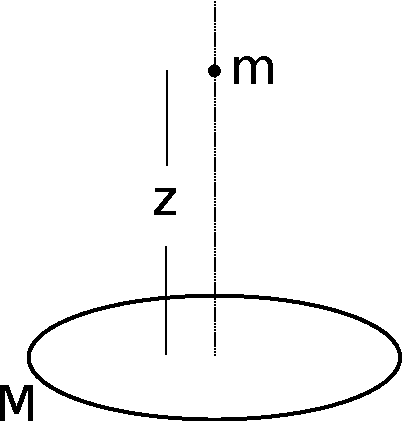
\includegraphics[width=0.45\textwidth,keepaspectratio]{aux/potencial_espira.pdf}
    \caption{Partícula de massa $m$ sobre um arame circular homogêneo
      de massa $M$.}
    \label{fig:potencial_espira}
  \end{figure}
\end{ex}

\begin{ex}
  \label{ex:potencial.casca}
  Considere uma partícula de massa $m$ e uma casca esférica homogênea
  de massa $M$ e raio $R$ como ilustrado na
  figura~\ref{fig:potencial_esfera}). Mostre que a energia potencial
  gravitacional da partícula é dada por
  $$V_g=
  \begin{cases}
    -\frac{GMm}{z}&\text{se $z\ge R$}\\
    -\frac{GMm}{R}&\text{se $z<R$.}
  \end{cases}
  $$

  \noindent\textit{Dica:} Defina a densidade de massa
  $\sigma=M/4\pi R^2$. Considere uma fita circular de raio
  $R\sen\theta$ e largura $R\Delta\theta$, onde $\theta$ é o ângulo
  que eixo vertical e o raio da casca fazem quando ele aponta para um
  ponto da fita. A massa dessa fita é
  $\Delta M=\sigma(2\pi R\sen\theta)R\Delta\theta$. A distância entre
  o centro da fita e a partícula é $z-R\cos\theta$. Usando o resultado
  do exercício anterior, mostre que a energia potencial gravitacional
  da partícula é dada por
  $$V_g=-\int_0^{\pi}\frac{2\pi Gm\sigma R^2\sin\theta}{\sqrt{R^2+z^2-2Rz\cos\theta}}\,d\theta\,.$$
  Use a mudança de variável $u=R^2+z^2-2Rz\cos\theta$ na integral para
  chegar na expressão
  $$V_g=-\frac{\pi Gm\sigma R}{z}\int_{R^2+z^2-2Rz}^{R^2+z^2+2Rz}\frac{du}{\sqrt{u}}\,.$$
  \begin{figure}[ht]
    \centering
    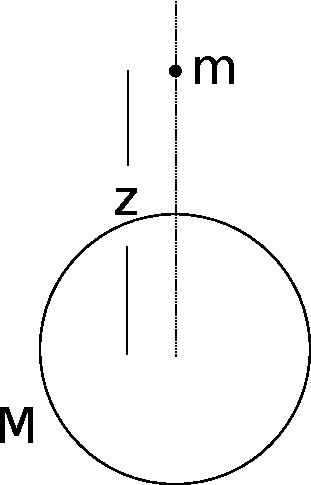
\includegraphics[width=0.45\textwidth,keepaspectratio]{aux/potencial_esfera.pdf}
    \caption{Partícula de massa $m$ sobre uma casca esférica homogênea
      de massa $M$.}
    \label{fig:potencial_esfera}
  \end{figure}
\end{ex}

\begin{ex}
  \label{ex:potencial.esfera}
  Considere agora que a figura~\ref{fig:potencial_esfera} se refere a
  uma esfera sólida de massa $M$ e raio $R$. Mostre que a energia
  potencial gravitacional da partícula é dada por
  $$V_g=
  \begin{cases}
    -\frac{GMm}{z}&\text{se $z\ge R$}\\
    2\pi Gm\sigma(\frac{z^2}{3}-R^2)&\text{se $z<R$.}
  \end{cases}
  $$

  \noindent\textit{Dica:} Defina a densidade de massa
  $\rho=\frac{M}{(4/3)\pi R^3}$. Considere uma casca esférica de raio
  $r$ e espessura $\Delta r$. A massa dessa casca é
  $\Delta M=\rho(4\pi r^2)\Delta r$. Usando o resultado do exercício
  anterior, mostre que, se $z\ge R$,
  $$V_g=-\int_0^R\frac{4\pi Gm\sigma r^2}{z}\,dr\,;$$
  se $z<R$,
  $$V_g=-\int_0^z\frac{4\pi Gm\sigma r^2}{z}\,dr-\int_z^R\frac{4\pi Gm\sigma r^2}{r}\,dr\,.$$
\end{ex}

\begin{ex}
  \label{ex:forca.esfera}
  Determine o módulo e a direção da força gravitacional sobre uma
  partícula de massa $m$ na situação dada no
  exercício~\ref{ex:potencial.casca} quando $z\ge R$ e quando
  $z<R$. Repita o mesmo para o caso do
  exercício~\ref{ex:potencial.esfera}. Mostre que seus resultados
  podem ser escritos de forma unificada como
  $$\vec F_g=-\frac{GM_{\mathrm{env}}m}{z^2}\hat k\,,$$
  onde $M_{\mathrm{env}}$ é a massa do corpo esférico que está envolta
  por uma esfera de raio $z$.
\end{ex}

Nos exercícios~\ref{ex:potencial.casca}, \ref{ex:potencial.esfera}
e~\ref{ex:forca.esfera} consideramos que a partícula se encontrava em
um ponto de uma linha vertical. No entanto, devido à simetria de um
corpo esférico, os resultados desses exercícios continuam valendo da
mesma forma desde que escolhamos o eixo $z$ como a semirreta que sai
do centro do corpo esférico e passa pela partícula.

Dos exercícios~\ref{ex:potencial.casca}, \ref{ex:potencial.esfera}
e~\ref{ex:forca.esfera} concluímos que para obter a energia potencial
ou a força gravitacional de um corpo qualquer localizado fora de um
outro corpo esférico homogêneo podemos considerar o segundo como uma
partícula localizada no seu centro de massa. Em particular, se
consideramos a Terra como uma esfera sólida homogênea, a energia
potencial gravitacional de uma partícula de massa $m$ que se encontra
a uma altura $h$ da superfície da Terra será
$$V_g=-\frac{GM_Tm}{R_T+h}\,,$$
onde $M_T$ e $R_T$ são respectivamente a massa e o raio da
Terra. Também podemos obter imediatamente que o valor da força
gravitacional sobre a partícula é
\begin{equation}
  \label{eq:12}
  F_g=\frac{GM_Tm}{(R_T+h)^2}\,,
\end{equation}
a qual aponta para o centro da Terra.

Considerando a Terra como uma esfera, o raio dela pode ser medido
experimentalmente de várias formas. Nós vamos considerar que o raio da
Terra é
$$R_T=6380\,\mathrm{km}\,.$$

Se uma partícula de massa $m$ se encontra a uma altura $h\ll R_T$ em
relação à superfície da Terra, a força gravitacional sobre a partícula
é chamada de \textbf{peso}. Nesse caso, o peso da partícula segundo a
Eq.~(\ref{eq:12}) vai ser aproximadamente
$$F_g=\frac{GM_Tm}{R_T^2}\,.$$
Por outro lado, nessa aproximação sabemos que $F_g=mg$, onde
$g=9{,}8\,\mathrm{m}/\mathrm{s}^2$. Logo, a partir dessas relações
podemos obter o valor da massa da Terra. De fato, vamos obter que
$M_T=5{,}98\times 10^{24}\,\mathrm{kg}$. O valor atualmente aceito
para a massa da Terra é
$$M_T=5.974\times 10^{24}\,\mathrm{kg}\,.$$

\begin{ex}
  Determine a velocidade mí\-ni\-ma que deve ser proporcionada a uma
  partícula de massa $m$, inicialmente sobre a superfície da Terra,
  para que ela se afaste da Terra e nunca volte. Essa velocidade é
  chamada de \textbf{velocidade de escape}.

  \noindent\textit{Dica:} A energia inicial da partícula é
  $$E_i=\frac{1}{2}mv^2-\frac{GM_Tm}{R_T}\,.$$
  A energia final da partícula, em uma posição infinitamente distante
  da Terra, é $E_f=0$ (velocidade final nula).
\end{ex}

\begin{ex}
  Uma partícula de massa $m$ se move uniformemente em uma órbita
  circular de raio $r$ em relação ao centro da Terra. Mostre que o
  módulo da velocidade da partícula deve ser dado por
  $$v=\sqrt{\frac{GM_T}{r}}\,.$$
  Definindo o \textbf{período} $T$ como o tempo que a partícula demora
  em dar uma volta na órbita, mostre que
  $$T=\frac{2\pi r^{3/2}}{\sqrt{GM_T}}\,.$$

  \noindent\textit{Dica:} A força gravitacional sobre a partícula é a
  força centrípeta. Logo,
  $$\frac{GM_Tm}{r^2}=ma_c\,,$$
  onde $a_c$ é a aceleração centrípeta.
\end{ex}

\begin{ex}
  Encontre qual é a velocidade que deve ser proporcionada a uma
  partícula de massa $m$, inicialmente na superfície da Terra, para
  que ela se mova em uma órbita circular de raio $r$ em relação ao
  centro da Terra.

  \noindent\textit{Dica:} Use o teorema da conservação da energia
  junto com a velocidade obtida no exercício anterior.
\end{ex}

Quase 80 anos antes de Newton formular a lei da gravitação universal,
Kepler, baseado em dados observacionais sobre o movimento dos
planetas, obteve as seguintes leis empíricas:
\begin{enumerate}
\item Os planetas se movem em órbitas elípticas ao redor do Sol, o
  qual está localizado em um dos focos da elipse (ver
  figura~\ref{fig:orbitaeliptica}).
\item O vetor posição de um planeta em relação ao Sol varre áreas
  iguais em intervalos de tempo iguais (ver
  figura~\ref{fig:leikepler2}).
\item O período de um planeta é diretamente proporcional ao semi-eixo
  maior da sua órbita elíptica elevado ao expoente $3/2$.
\end{enumerate}
\begin{figure}[ht]
  \centering
  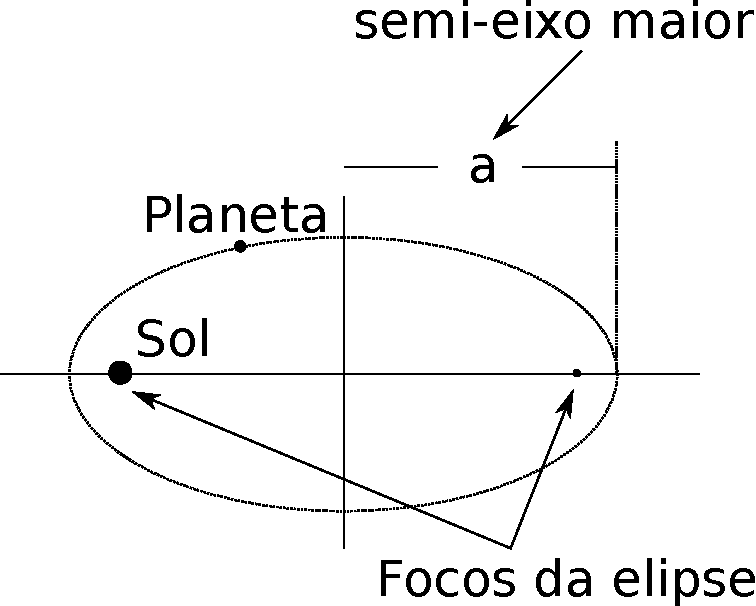
\includegraphics[width=0.45\textwidth,keepaspectratio]{aux/orbitaeliptica.pdf}
  \caption{Primeira lei de Kepler. Uma elipse tem a propriedade de
    que, para qualquer ponto dela, a soma das distâncias entre o ponto
    e os focos é uma constante.}
  \label{fig:orbitaeliptica}
\end{figure}
\begin{figure}[ht]
  \centering
  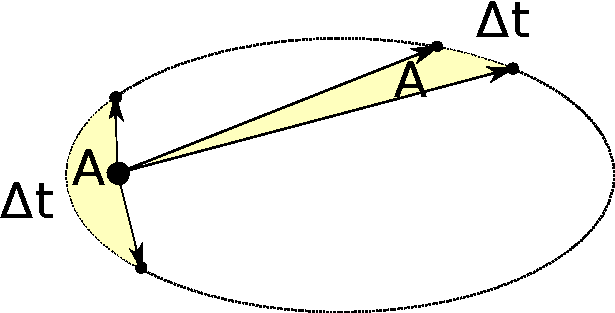
\includegraphics[width=0.45\textwidth,keepaspectratio]{aux/leikepler2.pdf}
  \caption{Segunda lei de Kepler.}
  \label{fig:leikepler2}
\end{figure}

Tendo formulado a lei da gravitação universal, Newton descobriu que a
partir dessa lei podem ser deduzidas as três leis de Kepler. As
deduções da primeira e da terceira leis usam manipulações de equações
diferenciais que estão fora do escopo do curso. A dedução da segunda
lei é mais elementar e veremos que é consequência da conservação do
momento angular.

Consideremos um planeta de massa $m$ a uma distância $r$ do centro do
Sol. Se $\vec F_g$ é a força gravitacional sobre o planeta devido ao
Sol, então o vetor $\vec F_g$ é proporcional ao vetor $-\vec r$. Dessa
maneira, o torque de $\vec F_g$ vai ser nulo, pois é o produto
vetorial de vetores paralelos. Se $\vec F_g$ é a única força que atua
sobre a planeta, segue então da Eq.~(\ref{eq:3}) que o momento angular
do planeta $\vec L=\vec r\times (m\dot{\vec r})$ se conserva, ou seja,
$\vec L$ é um vetor constante (módulo e direção constantes). Em
particular, isso implica que o vetor $\vec L$ vai ser sempre
perpendicular aos vetores $\vec r$ e $\dot{\vec r}$ e, por
conseguinte, o movimento do planeta é realizado em um plano que é
perpendicular a $\vec L$. Assim, podemos considerar convenientemente
que o plano do movimento é o plano $xy$ (ver
figura~\ref{fig:leikepler2r}).

\begin{figure}[ht]
  \centering
  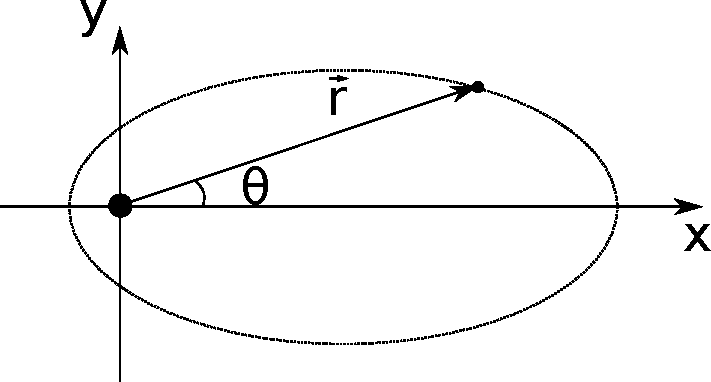
\includegraphics[width=0.5\textwidth,keepaspectratio]{aux/leikepler2r.pdf}
  \caption{O movimento do planeta é realizado no plano $xy$.}
  \label{fig:leikepler2r}
\end{figure}

Da figura~\ref{fig:leikepler2r} vemos que
$\vec r=r\cos\theta\hat i+r\sen\theta\hat j$. Logo,
\begin{equation*}
  \begin{split}
    \dot{\vec r}=(\dot r\cos\theta-r\dot\theta\sen\theta)\hat i+(\dot
    r\sen\theta+r\dot\theta\cos\theta)\hat j
  \end{split}
\end{equation*}
e, por conseguinte,
\begin{equation*}
  \begin{split}
    \vec L&=m\vec r\times\dot{\vec r}\\
    &=m\!\left|
      \begin{array}{ccc}
        \hat i&\hat j&\hat k\\
        r\cos\theta& r\sen\theta& 0\\
        \dot r\cos\theta\!-\!r\dot\theta\sen\theta& \dot r\sen\theta\!+\!r\dot\theta\cos\theta&0
      \end{array}
    \right|.
  \end{split}
\end{equation*}
Portanto,
\begin{equation*}
  \begin{split}
    \vec L&=m[r\cos\theta(\dot r\sen\theta+r\dot\theta\cos\theta)\\
    &\qquad-r\sen\theta(\dot r\cos\theta-r\dot\theta\sen\theta)]\hat k\\
    &=mr^2\dot\theta\hat k\,.
  \end{split}
\end{equation*}
Como esse vetor é constante, seu módulo $L=mr^2\dot\theta$ é uma
constante. Por outro lado, sabe-se dos cursos de cálculo que a área da
região limitada pela elipse e os vetores $\vec r(\theta_1)$ e
$\vec r(\theta_2)$ é dada por
$$A=\frac{1}{2}\int_{\theta_1}^{\theta_2}r^2\,d\theta\,.$$
Se $\theta_1=\theta(t_1)$ e $\theta_2=\theta(t_2)$, mudando a variável
de integração para $t$, temos que
$$A=\frac{1}{2}\int_{t_1}^{t_2}r^2\frac{d\theta}{dt}\,dt=\frac{1}{2}\int_{t_1}^{t_2}r^2\dot\theta\,dt=\frac{1}{2}\int_{t_1}^{t_2}\frac{L}{m}\,dt$$
Logo, como $L$ é constante, temos que
$$A=\frac{L}{2m}(t_2-t_1)\,.$$
Dessa maneira fica provada a segunda lei de Kepler, pois a área
varrida pelo vetor posição do planeta entre dois instantes de tempo
$t_1$ e $t_2$, só depende da diferença $t_2-t_1$ e não dos instantes
individuais.

Usando a lei da gravitação de Newton, a terceira lei de Kepler pode
ser formulada mais precisamente pela seguinte equação:
$$T=\frac{2\pi a^{3/2}}{\sqrt{GM_S}}\,,$$
onde $T$ é o período do planeta, $a$ é o comprimento do semi-eixo
maior da sua órbita e $M_S=1{,}99\times 10^{30}\,\mathrm{kg}$ é a
massa do Sol.

\begin{ex}
  O cometa Halley se move em uma órbita elíptica ao redor do Sol. No
  instante em que o cometa está mais próximo do Sol
  (\textbf{perihélio}), a distância entre o cometa e o Sol é de
  $8{,}75\times 10^7\,\mathrm{km}$. No instante em que o cometa está
  mais afastado do Sol (\textbf{afélio}), a distância entre o cometa e
  o sol é de $5{,}26\times 10^9\,\mathrm{km}$. Encontre o comprimento
  do semi-eixo maior da órbita e o período do cometa.
\end{ex}

As leis de Kepler, na forma em que foram anunciadas acima, valem sob a
condição de que a massa do Sol é muito maior do que a massa dos
planetas. De fato, a massa do Sol é maior do que a soma das massas dos
planetas. Nesse caso, o Sol fica praticamente em repouso enquanto os
planetas se movem. No entanto, em um sistema solar onde um planeta
tenha uma massa comparável com a do Sol, o Sol também se move. Nesse
caso, ambos corpos se movem em órbitas elípticas ao redor do centro de
massa. Omitindo a demonstração, afirmamos que as leis de Kepler
continuam valendo para o movimento relativo. O único detalhe é que a
terceira lei de Kepler é enunciada na seguinte forma:
$$T=\frac{2\pi a^{3/2}}{\sqrt{G(M_S+m)}}$$
onde $m$ é a massa do planeta.

\section{Movimento periódico}
Uma partícula realiza um movimento \textbf{periódico} se para qualquer
instante $t$ seus vetores posição e velocidade satisfazem as condições
\begin{equation}
  \label{eq:13}
  \vec r(t+c)=\vec r(t)\quad\text{e}\quad\vec v(t+c)=\vec v(t)
\end{equation}
para algum número $c\ne 0$. O menor número $c\ne 0$ para o qual as
Eqs.~(\ref{eq:13}) são satisfeitas é chamado de \textbf{período} da
partícula (ou do movimento) e é usualmente denotado por $T$. A unidade
de período no SI é o segundo ($s$).

Define-se a \textbf{frequência} do movimento como o inverso do
período, ou seja, $f=1/T$. A unidade de frequência no SI é o
\textbf{Hertz} ($\mathrm{Hz}$).

Exemplos de movimentos periódicos são os seguintes:
\begin{enumerate}
\item O movimento circular uniforme de uma partícula.
\item O movimento de um planeta em uma órbita ao redor do Sol.
\item O movimento horizontal de um bloco, acoplado a uma mola fixa
  sobre uma superfície lisa.
\item O movimento de uma partícula suspensa por uma corda unicamente
  sob o efeito da gravidade da Terra.
\item O movimento de um corpo rígido suspenso a partir de um ponto
  unicamente sob o efeito da gravidade da Terra.
\end{enumerate}

Vamos estudar o movimento oscilatório (vaivém) de um bloco acoplado a
uma mola fixa de massa desprezível, como mostrado na
figura~\ref{fig:massamola}. A posição de equilíbrio indicada na figura
representa a posição do bloco quando a mola não está deformada (não
está esticada nem comprimida). Quando o bloco está à direita da
posição de equilíbrio, ele estica a mola e, por conseguinte, a mola
exerce uma força sobre o bloco orientada para a esquerda. Quando o
bloco está à esquerda da posição de equilíbrio, ele comprime a mola e
devido a isso a mola exerce uma força sobre o bloco orientada para a
direita. Em ambos os casos a força aplicada pela mola tenta restituir
a forma da mola, por isso às vezes essa força é chamada de
\textbf{força de restituição}.
\begin{figure}[ht]
  \centering
  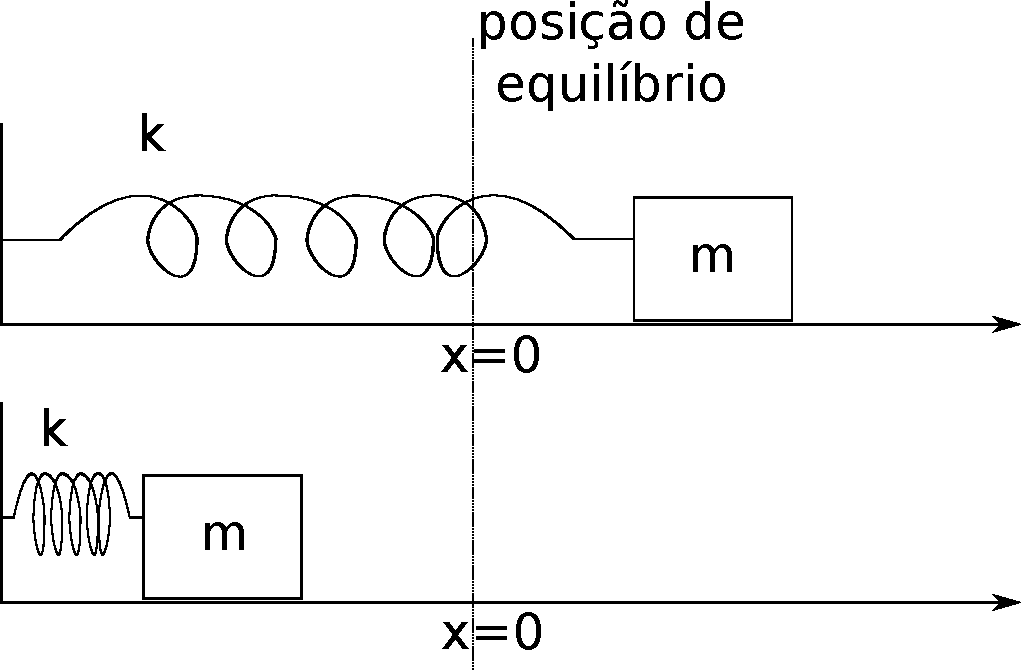
\includegraphics[width=0.45\textwidth,keepaspectratio]{aux/massamola.pdf}
  \caption{Movimento oscilatório de um bloco acoplado a uma mola
    fixa.}
  \label{fig:massamola}
\end{figure}

Se o bloco está em uma posição $x$, segundo a lei de Hooke, a força de
restituição sobre a o bloco é dada por $F=-kx$. Essa expressão vale
quando o bloco estica a mola ($x>0$) assim como quando o bloco
comprime a mola ($x<0$). Como a força de restituição é a força
resultante sobre o bloco, pela segunda lei de Newton, temos que
$$-kx=ma\,,$$
onde $a$ é a aceleração do bloco. Como $a=\dot v$ e $v=\dot x$, segue
que $a=\ddot x$ (segunda derivada de $x$ em relação a $t$). Logo,
obtemos a equação diferencial
\begin{equation}
  \label{eq:14}
  \ddot x+\frac{k}{m}x=0\,,
\end{equation}
que é chamada de equação do \textbf{oscilador harmônico
  simples}. Nesses termos, o bloco da figura~\ref{fig:massamola} é
chamado de um \textbf{oscilador harmônico}.

Existem vários métodos para resolver a Eq.~(\ref{eq:14}) que podem ser
estudados nos cursos de cálculo. No entanto, é possível obter-se a
forma de uma solução dessa equação de uma maneira simples relacionando
o movimento do oscilador harmônico com o movimento circular uniforme
de uma partícula.

Consideremos uma partícula que descreve uma trajetoria circular de
raio $A$ e se move uniformemente com velocidade $v$, como mostrado na
figura~\ref{fig:ociladoranalogia}. Nota-se dessa figura que a sombra
da partícula realiza um movimento horizontal oscilatório. Se $x=0$ é a
posição da origem do círculo e a partícula se encontra na posição
indicada na figura, vemos que sua sombra estará localizada na posição
\begin{equation}
  \label{eq:15}
  x=A\cos\theta\,.
\end{equation}
Como a partícula se move com velocidade angular constante
$\omega=\Delta\theta/\Delta t$, segue que
\begin{equation}
  \label{eq:16}
  \theta=\omega t+\phi\,,
\end{equation}
onde $\phi=\theta(0)$ é o ângulo de partida. Logo, segue das
Eqs.~(\ref{eq:15}) e~(\ref{eq:16}) que
\begin{equation}
  \label{eq:17}
  x=A\cos(\omega t+\phi).
\end{equation}

\begin{figure}[ht]
  \centering
  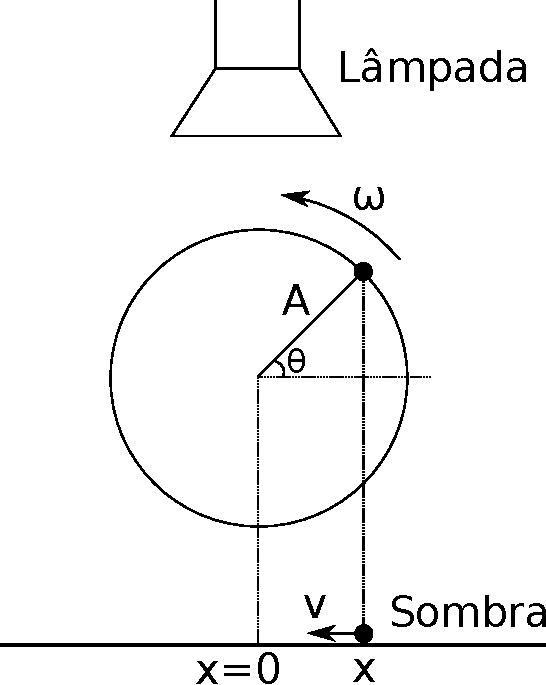
\includegraphics[width=0.45\textwidth,keepaspectratio]{aux/osciladoranalogia.pdf}
  \caption{Relação entre movimento circular uniforme e movimento de um
    oscilador harmônico.}
  \label{fig:ociladoranalogia}
\end{figure}

Pode-se perceber que o movimento descrito pela sombra da partícula da
figura~\ref{fig:ociladoranalogia} é similar ao movimento do oscilador
harmônico da figura~\ref{fig:massamola}. Como o último é descrito pela
Eq.~(\ref{eq:14}), podemos procurar uma solução dessa equação da forma
dada na Eq.~(\ref{eq:17}). Substituindo então~(\ref{eq:17})
em~(\ref{eq:14}) temos que
$$-A\omega^2\cos(\omega t+\phi)+\frac{k}{m}A\cos(\omega t+\phi)=0\,,$$
o qual é verdadeiro para quaisquer valores de $x$ e $t$ se, e somente
se, $\omega=\sqrt{k/m}$. Portanto, uma solução da equação do oscilador
harmônico~(\ref{eq:14}) é
\begin{equation}
  \label{eq:18}
  x=A\cos(\omega t+\phi)\,,\quad \text{com}\quad \omega=\sqrt{\frac{k}{m}}\,.
\end{equation}
De acordo com a teoria de equações diferenciais ordinárias, a solução
dada na Eq.~(\ref{eq:18}) é a chamada \textbf{solução geral} da
Eq.~(\ref{eq:14}), pois depende de duas constantes $A$ e $\phi$ a
serem determinadas. Como veremos depois, essas constantes podem ser
obtidas a partir do conhecimento da posição e da velocidade iniciais
do bloco, as quais são chamadas de \textbf{condições iniciais}.

Se a Eq.~(\ref{eq:18}) é a posição de um oscilador harmônico, sua
velocidade é dada por
\begin{equation}
  \label{eq:19}
  v=\dot x=-A\omega\sen(\omega t+\phi)\,.
\end{equation}
Se no instante inicial o oscilador está na posição $x_0$ e tem
velocidade $v_0$, segue das Eqs.~(\ref{eq:18}) e~(\ref{eq:19}) que
$x_0=A\cos\phi$ e $v_0=-A\omega\sen\phi$, ou, escrito de outra forma,
\begin{equation}
  \label{eq:20}
  x_0=A\cos\phi\quad\text{e}\quad \frac{v_0}{\omega}=-A\sen\phi\,.
\end{equation}
Elevando essas equações ao quadrado e somando-as, obtemos que
$$x_0^2+\frac{v_0^2}{\omega^2}=A^2(\cos^2\phi+\sen^2\phi)=A^2\,.$$
Portanto,
\begin{equation}
  \label{eq:21}
  A=\sqrt{x_0^2+\frac{v_0^2}{\omega^2}}\,.
\end{equation}
Vemos que $A\ge 0$ e que a igualdade acontece se $x_0=0$ e $v_0=0$
(nesse caso o bloco não se move e fica na posição de
equilíbrio). Logo, se $A>0$, segue da Eq.~(\ref{eq:20}) que
$$\phi=\arccos\frac{x_0}{A}\,.$$

A Eq.~(\ref{eq:18}) junto com as condições iniciais contêm toda a
informação sobre o movimento de um oscilador harmônico. Em particular,
deve ser possível verificar a partir daqui que o movimento do
oscilador é limitado e periódico. Com efeito, segue da
Eq.~(\ref{eq:18}) que $|x|\le A$ para qualquer instante $t$, pois a
$-1\le \cos z\le 1$ para qualquer $z$. Logo, a posição do oscilador só
pode assumir valores no intervalo $[-A,A]$. Por essa razão, a
constante $A$ é chamada de \textbf{amplitude} do oscilador harmônico
(maior valor para a posição do oscilador). Por outro lado, as funções
cosseno e seno tem período $2\pi$ (ver figura~\ref{fig:senocosseno}),
ou seja, o menor valor de $p$ tal que $\cos(z+p)=\cos z$ e
$\sen(z+p)=\sen z$ para qualquer $z$ é $p=2\pi$. Logo, segue da
Eq.~(\ref{eq:18}) que, para qualquer $t$,
\begin{equation*}
  \begin{split}
    x\dpar{t+\frac{2\pi}{\omega}}&=A\cos\dsqr{\omega\dpar{t+\frac{2\pi}{\omega}}+\phi}\\
    &=A\cos(\omega t+\phi+2\pi)\\
    &=A\cos(\omega t+\phi)\\
    &=x(t)\,.
  \end{split}
\end{equation*}
De forma análoga vamos podemos verificar que $v(t+2\pi/\omega)=v(t)$
para qualquer $t$. Logo, o oscilador harmônico realiza um movimento
periódico com período
\begin{equation}
  \label{eq:22}
  T=\frac{2\pi}{\omega}=2\pi\sqrt{\frac{m}{k}}\,.
\end{equation}
\begin{figure}[ht]
  \centering
  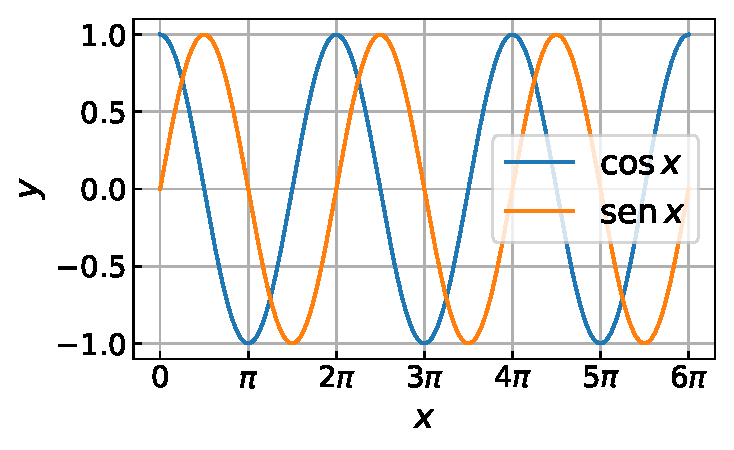
\includegraphics[width=0.45\textwidth,keepaspectratio]{aux/senocosseno.pdf}
  \caption{Gráficos das funções cosseno e seno.}
  \label{fig:senocosseno}
\end{figure}

O movimento que o oscilador realiza em um período é chamado de uma
única \textbf{oscilação} (ver
figura~\ref{fig:oscilador_periodo}). Lembrando que a frequência é o
inverso do período, segue que a frequência do oscilador é
\begin{equation}
  \label{eq:23}
  f=\frac{\omega}{2\pi}=\frac{1}{2\pi}\sqrt{\frac{k}{m}}\,.
\end{equation}
A frequência do oscilador nos dá o número de oscilações que o
oscilador realiza por unidade de tempo. Por outro lado, vemos da
Eq.~(\ref{eq:23}) que $\omega=2\pi f$. Se interpretamos $2\pi$ como o
ângulo associado a uma única oscilação, $\omega$ nos daria a variação
do ângulo associado por unidade de tempo. Isso justifica chamar a
grandeza $\omega$ de \textbf{frequência angular} do oscilador
harmônico.

\begin{figure}[ht]
  \centering
  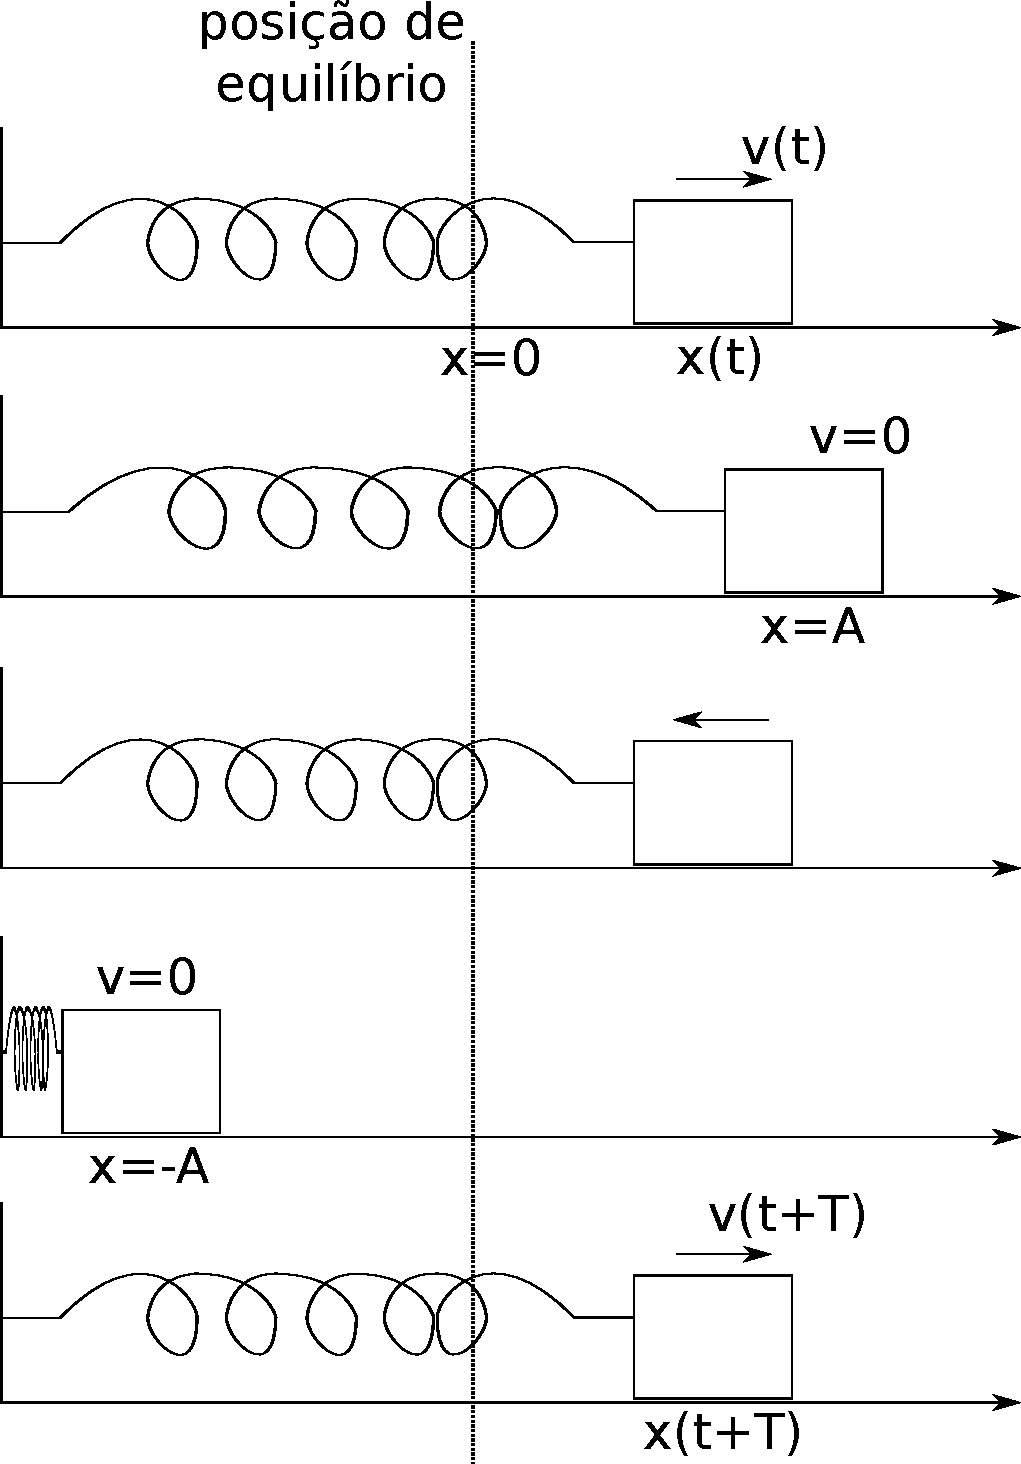
\includegraphics[width=0.45\textwidth,keepaspectratio]{aux/oscilador_periodo.pdf}
  \caption{Ilustração de uma única oscilação.}
  \label{fig:oscilador_periodo}
\end{figure}

A Eq.~(\ref{eq:22}) revela que o período de um oscilador harmônico é
diretamente proporcional à massa do oscilador elevada ao expoente
$1/2$. Isso faz sentido, pois, se o oscilador tem uma massa grande,
ele vai oferecer uma grande resistência a se mover e assim o tempo que
demorará para realizar uma única oscilação será também grande. Por
outro lado, a Eq.~(\ref{eq:22}) também expressa o fato de que o
período do oscilador é inversamente proporcional à constante elástica
da mola elevada ao expoente $1/2$. Isso também faz sentido, pois uma
constante elástica grande favorece o movimento do oscilador.

As Eqs.~(\ref{eq:22}) e~(\ref{eq:23}) nos dizem que o período e a
frequência (a frequência angular também) do oscilador harmônico não
dependem das condições iniciais, pois nessas equações não aparecem as
constantes $A$ e $\phi$. Isso quer dizer que, dados um oscilador de
massa $m$ e uma mola de constante $k$, não é possível mudar o tempo
que o oscilador demora em realizar uma única oscilação mudando a
posição e a velocidade iniciais do oscilador. No entanto, deve-se
ressaltar que a amplitude do oscilador depende das condições iniciais,
como fica evidente da Eq.~(\ref{eq:21}).

\begin{ex}
  Um bloco de $5\,\mathrm{kg}$ de massa está acoplado a uma mola fixa
  de constante elástica igual a $200\,\mathrm{N/m}$. Se inicialmente o
  bloco está esticando a mola e é liberado do repouso a uma distância
  de $0{,}5\,\mathrm{m}$ em relação à posição de equilíbrio da mola,
  encontre o período, a frequência e a frequência angular do
  bloco. Determine também a expressão da posição do bloco para
  qualquer instante de tempo $t$.
\end{ex}

\begin{ex}
  Considere o bloco e a mola do exercício anterior, mas agora suponha
  que no instante inicial o bloco está comprimindo a mola na posição
  $x_0=-0{,}2\,\mathrm{m}$ e tem velocidade
  $v_0=2\,\mathrm{m/s}$. Encontre o período, a frequência, a
  frequência angular e a amplitude do bloco.
\end{ex}

As forças que atuam sobre um oscilador harmônico são conservativas e,
por conseguinte, a energia total se conserva. Se a massa do oscilador
é $m$, a constante da mola é $k$, a posição do oscilador em relação à
posição de equlíbrio é $x$ e a velocidade do oscilador é $v$, então a
energia total do oscilador em um instante qualquer é dada por
$$E_T=\frac{mv^2}{2}+\frac{kx^2}{2}\,,$$
onde o segundo termo da direita corresponde à energia potencial
elástica. Como $x=A\cos(\omega t+\phi)$ e
$v=-A\omega\sen(\omega t+\phi)$, com $\omega=\sqrt{k/m}$, temos que
\begin{equation*}
  \begin{split}
    E_T&=\frac{m\omega^2A^2}{2}\sen^2(\omega t+\phi)+\frac{kA^2}{2}\cos^2(\omega t+\phi)\\
    &=\frac{kA^2}{2}[\sen^2(\omega t+\phi)+\cos^2(\omega t+\phi)]\,.
  \end{split}
\end{equation*}
Portanto,
$$E_T=\frac{kA^2}{2}\,,$$
que é uma constante.

\begin{ex}
  Um bloco de $2\,\mathrm{kg}$ de massa está acoplado a uma mola fixa
  de constante elástica igual a $100\,\mathrm{N/m}$. Se inicialmente o
  bloco está esticando a mola e é liberado do repouso a uma distância
  de $0{,}2\,\mathrm{m}$ em relação à posição de equilíbrio da mola,
  determine as velocidades que o bloco pode ter quando está nas
  posições $x=0\,\mathrm{m}$ e $x=0{,}1\,\mathrm{m}$.
\end{ex}

\begin{ex}
  Um bloco de massa $M$ está acoplado a uma mola fixa de constante
  elástica $k$. Suponha que o bloco oscila, tem amplitude $A_1$ e a
  velocidade do bloco quando passa pela posição de equilíbrio tem
  módulo igual a $v_1$. Se no instante em que o bloco passa pela
  posição de equilíbrio, uma massinha de massa $m$, inicialmente em
  repouso se gruda ao bloco, determine o novo período e a nova
  amplitude do movimento.

  \noindent\textit{Dica:} Para encontrar a velocidade $v_2$ que o
  sistema $\text{bloco}\,+\,\text{massinha}$ tem depois da colisão
  entre os dois corpos, use conservação do momento linear total.
\end{ex}

\begin{ex}
  Considere um bloco de massa $m$ unido ao extremo de uma mola de
  constante elástica $k$ que está na posição vertical e cujo outro
  extremo está fixo no teto. (i) Se $y=0$ corresponde à posição do
  bloco quando ele está em equilíbrio (força resultante nula),
  encontre a posição do bloco para a qual a mola não está
  deformada. (ii) Aplique a segunda lei de Newton sobre o bloco e
  mostre que a equação diferencial que descreve o movimento do bloco é
  igual à equação do oscilador harmônico simples. Daqui conclua que o
  movimento do bloco é periódico e que sua frequência angular é
  $\sqrt{k/m}$.
\end{ex}

\begin{ex}
  Uma balança de açougueiro consiste em uma plataforma de
  $0{,}2\,\mathrm{kg}$ suspensa por uma mola de massa desprezível de
  constante elástica $k=400\,\mathrm{N/m}$. Em um determinado instante
  um pedaço de carne de $2{,}2\,\mathrm{kg}$ é largado do repouso a
  uma altura de $0{,}4\,\mathrm{m}$ em relação à plataforma. Depois
  que a carne colide com a plataforma, os dois corpos ficam grudados e
  oscilam juntos. Determine o período e a amplitude do movimento.
\end{ex}

\begin{ex}
  Um \textbf{pêndulo simples} é composto por uma partícula de massa
  $m$ suspensa por uma corda sem massa de comprimento $l$, a qual tem
  um dos seus extremos fixo (no teto, por exemplo). Usando a segunda
  lei de Newton, mostre que a equação diferencial que descreve o
  movimento da partícula é
  $$\ddot\theta+\frac{g}{l}\sen\theta=0\,,$$
  onde $\theta$ é o ângulo que a corda faz com a vertical. Se $\theta$
  é pequeno ($\le 15º$), podemos usar a aproximação
  $\sen\theta\approx \theta$. Nesse caso, a equação diferencial
  anterior pode ser escrita de forma aproximada como
  $$\ddot\theta+\frac{g}{l}\theta=0\,.$$
  Conclua daqui que o movimento da partícula é oscilatório e
  periódico. Além disso, mostre que o período do movimento é dado por
  $$T=2\pi\sqrt{\frac{l}{g}}\,,$$
  o qual não depende da massa da partícula e nem das condições
  iniciais.
\end{ex}

\begin{ex}
  Um \textbf{pêndulo físico} consiste em um corpo rígido de massa $M$
  e momento de inércia $I$ suspenso por um ponto $O$ do corpo,
  diferente do centro de massa. Se $\theta$ é o ângulo que o segmento
  que une os pontos $O$ e o centro de massa faz com a vertical, usando
  as equações $\vec\tau_\mathrm{ext}=\dot{\vec L}$ e $L=I\dot\theta$,
  mostre que a equação que descreve o movimento do pêndulo físico é
  $$\ddot\theta+\frac{MgR}{I}\sen\theta=0\,,$$
  onde $R$ é o comprimento de tal segmento. Mostre que se $\theta$ é
  pequeno, o movimento do pêndulo físico é oscilatório e
  aproximadamente periódico, com período
  $$T=2\pi\sqrt{\frac{I}{MgR}}\,.$$
\end{ex}

\begin{ex}
  Considere uma barra homogênea de comprimento $l$ suspensa por um dos
  seus extremos. Se a barra é liberada do repouso fazendo um ângulo
  pequeno com a vertical, mostre que o movimento da barra é
  oscilatório e periódico, com período
  $$T=2\pi\sqrt{\frac{2l}{3g}}$$
\end{ex}

Em situações do dia a dia, quando um corpo realiza um movimento
oscilatório, observa-se que a amplitude do movimento diminui com o
tempo. Isso se deve à presença de forças de atrito ou forças de
resistência (forças dissipativas) que atuam sobre o corpo. Em
determinados casos, por exemplo quando o corpo está embebido em um
fluido (por exemplo, ar, óleo, etc.) a força de atrito sobre o corpo
tem módulo proporcional à velocidade do corpo. Consideremos, por
exemplo, um bloco de massa $m$, sobre uma mesa lisa, acoplado a um dos
extremos de uma mola sem massa de constante elástica $k$, cujo outro
extremo está fixo. Suponhamos que o ar aplica sobre o bloco uma força
de resistência $-bv$ ($b>0$), onde $v$ é a velocidade do bloco. Logo,
aplicando a segunda lei de Newton, vamos obter que
\begin{equation}
  \label{eq:24}
  \ddot x+\frac{b}{m}\dot x+\frac{k}{m}x=0\,.
\end{equation}
Vemos que a única diferença entre essa equação e a do oscilador
harmônico simples é o termo $b\dot x/m$. Pode-se provar, usando a
teoria de equações diferenciais que, se $b<2\sqrt{km}$, a solução da
Eq.~(\ref{eq:24}) é
\begin{equation}
  \label{eq:25}
  x=Ae^{-bt/2m}\cos(\omega' t+\phi)\,,
\end{equation}
onde $A$ e $\phi$ são constantes a serem determinadas pelas condições
iniciais e
\begin{equation}
  \label{eq:26}
  \omega'=\sqrt{\frac{k}{m}-\frac{b^2}{4m^2}}\,.
\end{equation}

A Eq.~(\ref{eq:25}) nos diz que, no caso em que a força de atrito é
pouco intensa ($b<2\sqrt{km}$), o bloco realizará oscilações com
amplitudes cada vez menores. Mais precisamente a amplitude do bloco
decairá de forma exponencial, devido ao fator $e^{-bt/2m}$ na
Eq.~(\ref{eq:25}).  Se incrementamos o valor de $b$ de tal forma que
tenhamos $b=2\sqrt{km}$, vemos da Eq.~(\ref{eq:26}) que $\omega'=0$ o
que significa que o bloco não oscila mais e a posição do bloco vai
rapidamente à posição de equilíbrio. A condição $b=2\sqrt{km}$ é
chamada de \textbf{amortecimento crítico}. Essa situação é a ideal
para o funcionamento do amortecedor de um carro.

Se $b>2\sqrt{km}$, a Eq.~(\ref{eq:25}) não é mais solução da
Eq.~(\ref{eq:24}) devido a que, na Eq.~(\ref{eq:26}), $\omega'$
torna-se um número imaginário. Nesse caso, a teoria das equações
diferenciais nos diz que a solução da Eq.~(\ref{eq:24}) é da forma
\begin{equation}
  \label{eq:27}
  x=Ae^{-a_1t}+Be^{-a_2t}\,,
\end{equation}
onde $A$ e $B$ são constantes determinadas pelas condições iniciais e
$a_1$ e $a_2$ são constantes determinadas por $k,m$ e $b$. Segue da
Eq.~(\ref{eq:27}) que, similarmente ao caso do amortecimento crítico,
o bloco não oscila. No entanto, a posição do bloco assume a posição de
equilíbrio com uma rapidez menor do que no caso anterior. A condição
$k>2\sqrt{km}$ é chamada de \textbf{superamortecimento}. Nessa
direção, a condição $k<2\sqrt{km}$ é chamada de
\textbf{subamortecimento}. A figura~\ref{fig:osciladoramortecido}
ilustra a posição de um oscilador harmônico amortecido para cada
instante de tempo nas três condições de amortecimento.

\begin{figure}[ht]
  \centering
  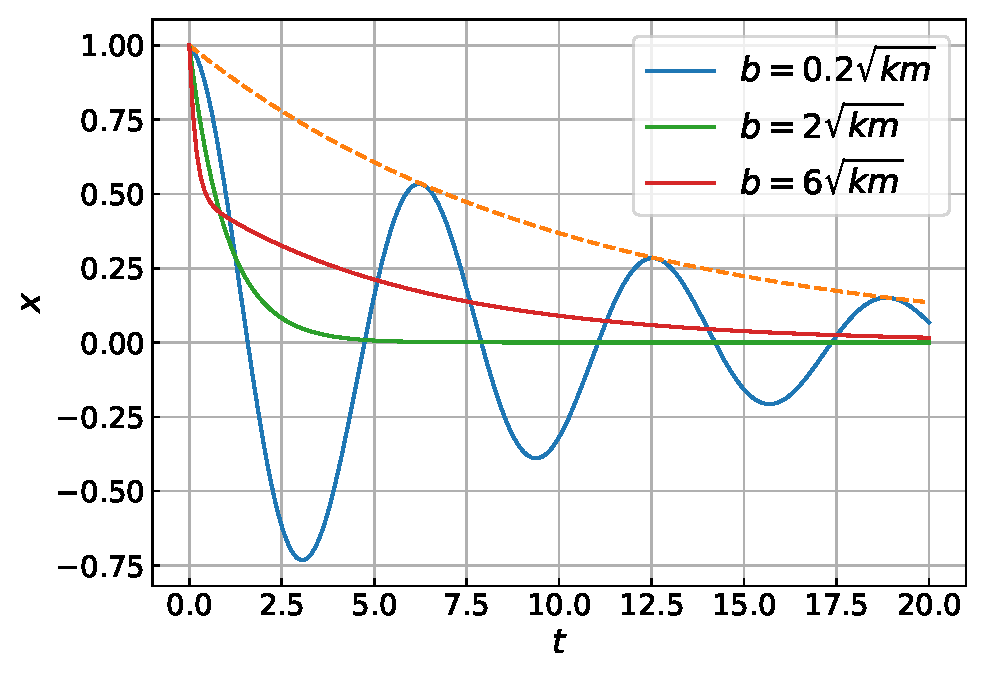
\includegraphics[width=0.45\textwidth,keepaspectratio]{aux/osciladoramortecido.pdf}
  \caption{Gráfico da posição de um oscilador harmônico amortecido nos
    casos subamortecido ($b=0{,}2\sqrt{km}$), críticamente amortecido
    ($b=2\sqrt{km}$) e superamortecido ($b=6\sqrt{km}$).}
  \label{fig:osciladoramortecido}
\end{figure}

Vejamos o que acontece com a energia total de um oscilador harmônico
amortecido, descrito pela Eq.~(\ref{eq:24}). A energia total em um
instante qualquer é dada por
$$E_T=\frac{mv^2}{2}+\frac{kx^2}{2}\,.$$
Logo, a derivada da energia total em relação ao tempo é
$$\dot E_T=mv\dot v+kx\dot x\,.$$
Usando o fato de que $v=\dot x$, temos que
$$\dot E_T=\dot x(m\ddot x+kx)\,.$$
Finalmente usando a Eq.~(\ref{eq:24}) obtemos que
$$\dot E_T=-b\dot x^2<0\,,$$
o que quer dizer que a energia total diminui com o tempo, o qual é
esperado devido à presença de forças dissipativas.

Para acabar com essa seção vamos considerar o caso em que uma força
externa $F$ é aplicada sobre um oscilador harmônico amortecido. Nesse
caso, a Eq.~(\ref{eq:24}) assume a forma
$$\ddot x+\frac{b}{m}\dot x+\frac{k}{m}x=\frac{F}{m}\,.$$
O caso mais interessante é quando o valor da força $F$ oscila no tempo
com uma frequência angular $\omega_F$, ou seja,
$F=F_0\cos\omega_Ft$. Pode-se mostrar que nesse caso, a amplitude do
oscilador é dada por
$$A=\frac{F_0}{\sqrt{(k-m\omega_F^2)^2+b^2\omega_F^2}}\,.$$
Vemos daqui que a amplitude é máxima quando $\omega_F=\sqrt{k/m}$, e
nesse caso, $A=\frac{F_0}{b}\sqrt{\frac{m}{k}}$. Se $b$ é pequeno (por
exemplo, no caso de subamortecimento) o valor máximo da amplitude pode
ser bastante grande e corresponde a um pico pronunciado no gráfico $A$
versus $\omega_F$. Quando o sistema se encontra nessa situação
extrema, dizemos que ocorreu \textbf{ressonância}.

\section{Ondas mecânicas}

Uma \textbf{onda mecânica} é uma perturbação que se desloca através de
um material (uma corda, o ar, a água, etc.), chamado de \textbf{meio}
de propagação da onda. Conforme a onda se propaga através do meio, as
partículas do meio sofrem deslocamentos. Esses deslocamentos podem ser
perpendiculares à direção de propagação da onda, como no caso de uma
onda que se propaga através de uma corda tensionada, podem ser
paralelos, como no caso do som que se propaga no ar, ou a combinação
dos dois, como no caso de uma onda que se propaga através superfície
de um líquido. No primeiro caso a onda é chamada de uma \textbf{onda
  transversal} e no segundo de uma \textbf{onda longitudinal} (no
último caso a onda tem uma componente tranversal e outra
longitudinal).

Antes de uma onda se propagar através de um méio, as partículas do
meio não foram perturbadas ainda e se encontram em posições de
equilíbrio. Quando a onda se propaga, as partículas do meio se
deslocam e aparecem forças de restituição que tentam fazer as
partículas do meio voltarem às suas respectivas posições de
equilíbrio. Dessa maneira, as partículas do meio realizam movimentos
oscilatórios. Deve-se ressaltar que as velocidades das partículas do
meio são diferentes da velocidade de propagação da onda. Por outro
lado, como o movimento das partículas do meio é oscilatório, uma onda
não transporta matéria de uma região do meio para outra. No entanto,
como partículas do meio que estavam inicialmente em repouso começam a
oscilar (ganham energia) quando a onda passa, a onda transfere energia
de uma região do meio para outra.

Quando um meio é perturbado produzindo uma única ondulação que se
propaga através dele, a onda produzida é chamada às vezes de
\textbf{pulso ondulatório}. Por outro lado, se o meio é perturbado de
forma contínua e periódica, a onda produzida é chamada de \textbf{onda
  periódica}. Nesse caso, conforme a onda se propaga, as partículas do
meio realizam movimentos oscilatórios e periódicos que têm o mesmo
período.

Um caso importante de onda periódica ocorre quando a onda faz as
partículas do meio se comportarem como osciladores harmônicos simples
que têm a mesma frequência e a mesma amplitude. Nesse caso, a onda é
chamada de uma \textbf{onda senoidal}, pois tem a forma do gráfico das
funções trigonométricas seno ou cosseno (ver
figura~\ref{fig:onda}). Os pontos onde as partículas do meio sofreram
um deslocamento positivo (negativo) máximo devido a uma onda senoidal
são chamados de \textbf{cristas} (\textbf{vales}). O comprimento de
onda de uma onda senoidal pode ser obtido então medindo a distância
entre duas cristas (ou entre dois vales) consecutivos.

\begin{figure}[ht]
  \centering
  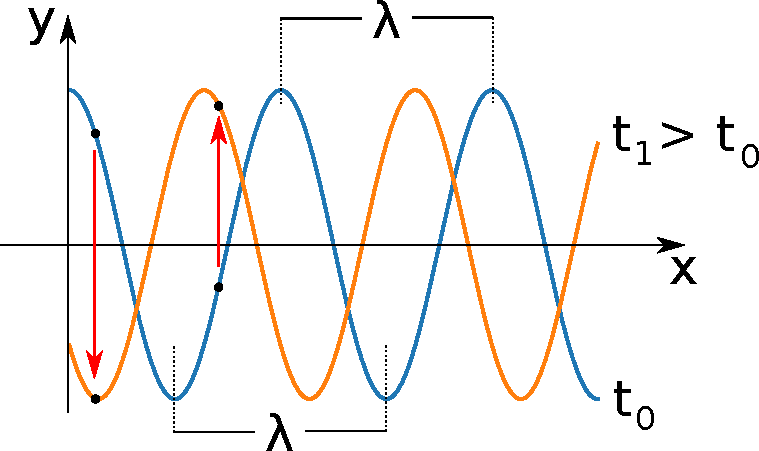
\includegraphics[width=0.45\textwidth,keepaspectratio]{aux/onda.pdf}
  \caption{Onda periódica de comprimento de onda $\lambda$ que se
    propaga para a direita através de uma corda em dois instantes de
    tempo $t_0$ e $t_1$. As setas em vermelho indicam os deslocamentos
    das partículas da corda provocados pela propagação da onda.}
  \label{fig:onda}
\end{figure}

A distância que uma onda periódica percorre em um intervalo de tempo
igual a um período é chamado de \textbf{comprimento de onda} e é
usualmente denotado por $\lambda$ (lê-se lambda). Conhecendo-se o
comprimento de onda $\lambda$ e o período $T$ de uma onda periódica, a
velocidade de propagação da onda pode ser encontrada pela relação
\begin{equation}
  \label{eq:28}
  v=\frac{\lambda}{T}=\lambda f\,,
\end{equation}
onde $f=1/T$ é a frequência da onda. Em muitos casos, a velocidade da
onda só depende das propriedades mecânicas do meio. Dessa maneira, a
Eq.~(\ref{eq:28}) implica que um aumento na frequência da onda produz
uma diminuição no seu comprimento de onda e vice-versa.

\begin{ex}
  \textbf{Ondas sonoras} são ondas longitudinais periódicas que se
  propagam no ar. A velocidade de propagação de uma onda sonora
  (velocidade do som) depende da temperatura do ambiente. Se a
  velocidade do som a $20\,º\mathrm{C}$ é 344\,\textrm{m/s}, determine
  o comprimento de onda de uma onda sonora de frequência igual a
  $784\,\mathrm{Hz}$ (Nota sol na quinta oitava de um piano).
\end{ex}

Ondas podem se propagar em mais de uma direção, por exemplo a onda
produzida na superfície de um líquido quando uma gota de água cai
sobre ela. No entanto, adotando um posto de vista introdutório, nós
estaremos interessados somente em ondas que se propagam em uma única
direção, a qual será identificada com o eixo $x$.

Como as partículas de um meio se comportam como osciladores harmônicos
simples que têm a mesma frequência angular $\omega$ e a mesma
amplitude $A$ quando uma onda senoidal se propaga, o deslocamento de
uma partícula na posição $x$ para qualquer instante de tempo $t$ será
dado por
\begin{equation}
  \label{eq:29}
  y(x,t)=A\cos(\omega t+c(x))\,,
\end{equation}
onde $c(x)$ é uma função de $x$. Em particular vamos ter que
$y(0,t)=A\cos(\omega t+c(0))$. Se a onda se propaga para a direita com
velocidade $v$, depois de um intervalo de tempo $x/v$, os
deslocamentos da partícula na posição $x\ge 0$ serão iguais que os
deslocamentos sofridos pela partícula na posição $x=0$. Logo, vamos
ter que
$$A\cos(\omega t+c(0))=A\cos\dpar{\omega\dpar{t+\frac{x}{v}}+c(x)}$$
para todo $t$. Essa igualdade é satisfeita se
$$\omega t+c(0)=\omega t+\frac{\omega}{v} x+c(x)\,,$$
ou seja, se
$$c(x)=c(0)-\frac{\omega}{v} x\,.$$
Substituindo isso na Eq.~(\ref{eq:29}) temos que
$$y(x,t)=A\cos\dpar{\omega t-\frac{\omega}{v} x+c(0)}\,.$$
Como o cosseno é uma função par ($\cos (-z)=\cos z$ para qualquer
$z$), então, pondo $c(0)=-\phi$, vamos ter que
\begin{equation}
  \label{eq:30}
  y(x,t)=A\cos(kx-\omega t+\phi)\,,
\end{equation}
onde
$$k=\frac{\omega}{v}$$
é chamado de \textbf{número de onda} ou \textbf{vetor de onda}. A
função $y$ dada pela Eq.~(\ref{eq:30}) é chamada de uma \textbf{função
  de onda}, a constante $A$ é chamada de \textbf{amplitude} da onda e
$\phi$ de \textbf{fase}. Pode-se verificar que, no caso de uma onda
senoidal que se propaga para à esquerda, o sinal de $\omega t$ na
Eq.~(\ref{eq:30}) é positivo.

\begin{ex}
  Se uma onda senoidal tem sua função de onda dada pela
  Eq.~(\ref{eq:30}), mostre que
  $$k=\frac{2\pi}{\lambda}\quad\text{e}\quad \omega=2\pi f\,,$$
  onde $\lambda$ é o comprimento de onda e $f$ a frequência da onda.

  \noindent\textit{Dica:} Use a periodicidade da função cosseno junto
  ao fato de que $y(x+n\lambda,t)=y(x,t)$ para qualquer $t$ e qualquer
  inteiro $n\ge 0$.
\end{ex}

\begin{ex}
  Uma onda transversal senoidal com amplitude igual a
  $0{,}02\,\mathrm{m}$ e comprimento de onda igual a
  $0{,}5\,\mathrm{m}$ se propaga através de uma corda tensionada de
  esquerda para a direita com velocidade de $10\,\mathrm{m/s}$. (i)
  Determine o número de onda, a frequência e a frequência angular da
  onda. (ii) Encontre a função de onda que descreve a onda sabendo que
  no instante inicial a extremidade da esquerda está na posição de
  equilíbrio e se move de cima para baixo. (iii) Encontre a expressão
  do deslocamento de um ponto da corda que está na posição
  $x=3\,\mathrm{m}$ para qualquer instante de tempo.
\end{ex}

A velocidade de uma partícula do meio pela qual passa uma onda
senoidal descrita pela função de onda~(\ref{eq:30}) é dada pela
derivada parcial de $y$ em relação ao tempo, ou seja,
$$\frac{\partial y}{\partial t}=\omega A\sen(kx-\omega t+\phi)\,.$$
Da mesma forma, a aceleração dessa partícula será dada por
\begin{equation}
  \label{eq:31}
  \frac{\partial^2 y}{\partial t^2}=\omega^2A\cos(kx-\omega t+\phi)=\omega^2y(x,t)\,.
\end{equation}
Por outro lado, a derivada parcial de $y$ em relação a $x$ é
$$\frac{\partial y}{\partial x}=-kA\sen(kx-\omega t+\phi)$$
e, por conseguinte,
\begin{equation}
  \label{eq:32}
  \frac{\partial^2 y}{\partial x^2}=k^2A\cos(kx-\omega t+\phi)=k^2y(x,t)\,.
\end{equation}
Vemos então das equações~(\ref{eq:31}) e~(\ref{eq:32}) que
$$\frac{1}{\omega^2}\frac{\partial^2 y}{\partial t^2}=\frac{1}{k^2}\frac{\partial^2 y}{\partial x^2}\,.$$
Lembrando que $\omega/k=v$, onde $v$ é a velocidade de propagação da
onda, obtemos a equação
\begin{equation}
  \label{eq:33}
  \frac{\partial^2 y}{\partial x^2}=\frac{1}{v^2}\frac{\partial^2 y}{\partial t^2}\,,
\end{equation}
a qual é chamada de \textbf{equação de onda}.

A função de onda~(\ref{eq:30}), que descreve uma onda senoidal, é uma
solução particular da equação de onda. A equação de onda admite outros
tipos de solução, por exemplo funções de onda que descrevem ondas
triangulares, quadradas, etc.

Suponhamos que uma onda transversal se propague através de uma corda
tensionada de densidade linear de massa $\rho(x)$ e consideremos uma
porção da corda como ilustrado na
figura~\ref{fig:ondavelocidade}. Desprezando o efeito da gravidade e
considerando que a corda se deforma muito pouco quando a onda passa,
as únicas forças que atuam sobre a porção de corda são as tensões
$\vec F(x)$, no seu extremo esquerdo, e $\vec F(x+\Delta x)$, no
direito. Logo, decompondo essas forças em componentes horizontal e
vertical e usando a segunda lei de Newton vamos ter que
$$F(x+\Delta x)\cos\theta(x+\Delta x)-F(x)\cos\theta(x)=0$$
e
\begin{multline*}
  F(x+\Delta x)\sen\theta(x+\Delta x)\\
  -F(x)\sen\theta(x)=\rho(x)\sqrt{\Delta x^2+\Delta
    y^2}\frac{\partial^2 y}{\partial t^2}\,.
\end{multline*}
Dividindo essas equações por $\Delta x$ e tomando o limite
$\Delta x\to 0$, vamos ter que
\begin{equation}
  \label{eq:34}
  \begin{split}
    \frac{\partial}{\partial x}[F\cos\theta]&=0\\
    \frac{\partial}{\partial
      x}[F\sen\theta]&=\rho(x)\sqrt{1+\dpar{\frac{\partial y}{\partial
          x}}^2}\frac{\partial^2 y}{\partial t^2}\,.
  \end{split}
\end{equation}
Como a corda se deforma muito pouco quando a onda se propaga, vamos
ter $|\partial y/\partial x|\ll 1$ e assim podemos usar a aproximação
$1+(\partial y/\partial x)^2\approx 1$. Por outro lado,
$\tan\theta=\partial y/\partial x$,
$$\cos\theta=\frac{1}{\sqrt{\sec^2\theta}}=\frac{1}{\sqrt{1+\tan^2\theta}}=\frac{1}{\sqrt{1+(\frac{\partial y}{\partial x})^2}}\approx 1$$
e
$$\sen\theta=\cos\theta\tan\theta\approx \frac{\partial y}{\partial x}\,.$$
Logo, nas equações~(\ref{eq:34}) vamos ter que
\begin{equation*}
  \begin{split}
    \frac{\partial F}{\partial x}&=0\\
    \frac{\partial F}{\partial x}\frac{\partial y}{\partial
      x}+F(x)\frac{\partial^2 y}{\partial
      x^2}&=\rho(x)\frac{\partial^2 y}{\partial t^2}\,.
  \end{split}
\end{equation*}
Portanto,
$$\frac{\partial^2 y}{\partial x^2}=\frac{\rho(x)}{F(x)}\frac{\partial^2 y}{\partial t^2}\,.$$
Comparando essa Eq. com a Eq. de onda~(\ref{eq:33}), obtemos que a
velocidade de propagação da onda através da corda é dada por
$$v(x)=\sqrt{\frac{F(x)}{\rho(x)}}\,.$$

\begin{figure}[ht]
  \centering
  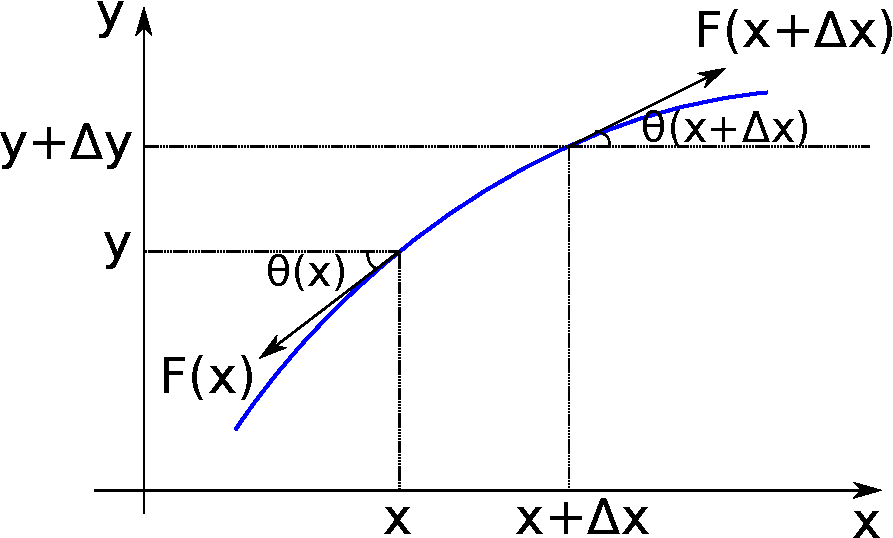
\includegraphics[width=0.45\textwidth,keepaspectratio]{aux/ondavelocidade.pdf}
  \caption{Porção de uma corda tensionada, pela qual se propaga uma
    onda transversal.}
  \label{fig:ondavelocidade}
\end{figure}

\begin{ex}
  \label{ex:ondapoco}
  João se encontra no fundo de um poço de $80\,\mathrm{m}$ de
  profundidade. Na sua posição se encontra um bloco de
  $15\,\mathrm{kg}$ suspenso por uma corda de $2\,\mathrm{kg}$, a qual
  conecta o bloco com um suporte que se encontra na superfície. Em um
  certo instante João balnça a corda gerando uma onda que se propaga
  de baixo para cima. (i) Assumindo que a tensão da corda é a mesma em
  todo ponto dela, calcule o tempo que a onda demora em chegar na
  superfície. (ii) Levando em conta que a tensão não é constante,
  determine a velocidade da onda quando ela chega na superfície.
\end{ex}

Uma onda transfere energia de uma região do méio para outra. Para
analisar essa transferência de energia, vamos considerar o caso
partícular de uma onda transversal que se propaga de esquerda para à
direita através de uma corda, a qual se deforma muito pouco. Nesse
caso, desprezando efeitos gravitacionais, a única força que atua sobre
a porção de corda constituida por pontos com posições $\ge x$ é a
tensão $\vec F(x)$. Essa força realiza um trabalho
$-F(x)\sen\theta(x)\Delta y$ sobre a porção de corda em
consideração. Logo, o trabalho realizado por unidade de tempo
(potência) será $-F(x)\sen\theta(x)\,(\Delta y/\Delta t)$. Tomando o
limite $\Delta t\to 0$, obtemos a potência instantânea
$$P(x,t)=-F(x)\sen\theta(x)\frac{\partial y}{\partial t}\,.$$
Como a corda se deforma pouco,
$\sen\theta\approx \partial y/\partial x$ e, por conseguinte,
\begin{equation}
  \label{eq:35}
  P(x,t)=-F(x)\frac{\partial y}{\partial x}\frac{\partial y}{\partial t}\,.
\end{equation}

A expressão da potência instantânea dada na Eq.~(\ref{eq:35}) é valida
para qualquer onda transversal que se propaga por uma corda, seja
senoidal ou não. Em particular, se a onda é senoidal e é descrita pela
função de onda $y(x,t)=A\cos(kx-\omega t+\phi)$, vamos ter que
$\partial y/\partial x=-kA\sen(kx-\omega t+\phi)$ e
$\partial y/\partial x=\omega A\sen(kx-\omega t+\phi)$. Logo, na
Eq.~(\ref{eq:35}) vamos ter que
$$P(x,t)=k\omega A^2F(x)\sen^2(kx-\omega t+\phi)\,.$$
Lembrando que $v=\omega/k=\sqrt{F(x)/\rho(x)}$, temos que
$k=\omega\sqrt{\rho(x)/F(x)}$. Portanto,
\begin{equation}
  \label{eq:36}
  P(x,t)=\sqrt{\rho(x)F(x)}\omega^2A^2\sen^2(kx-\omega t+\phi)\,.
\end{equation}
Segue daqui que a potência instantânea de uma onda senoidal nunca é
negativa. Isso quer dizer que se a energia flui de uma região do meio
para outra, o fluxo de energia segue o sentido da propagação da onda
senoidal e nunca no sentido contrário.

Como o valor máximo da função $\sen^2$ é $1$, segue da
Eq.~(\ref{eq:36}) que o valor máximo da potência instantânea é
$$P_\mathrm{max}(x)=\sqrt{\rho(x)F(x)}\omega^2A^2\,.$$
Por outro lado, a potência média é dada por
$$P_\mathrm{med}(x)=\frac{1}{T}\int_0^TP(x,t)\,dt\,,$$
onde $T$ é o período da onda. Logo,
$$P_\mathrm{med}(x)=\frac{P_\mathrm{max}(x)}{T}\int_0^T\sen^2(kx-\omega t+\phi)\,dt\,.$$
Usando a identidade trigonométrica $2\sen^2z=1-\cos 2z$, temos que
$$P_\mathrm{med}(x)=\frac{P_\mathrm{max}(x)}{2T}\int_0^T[1-\cos[2(kx-\omega t+\phi)]\,dt\,.$$
Logo,
$$P_\mathrm{med}(x)=\frac{P_\mathrm{max}(x)}{2T}\dsqr{t+\frac{\sen[2(kx-\omega t+\phi)]}{2\omega}}_0^T\,.$$
Como o segundo termo do lado direito dá o mesmo valor quando avaliado
nos limites, vamos obter que
$$P_\mathrm{med}(x)=\frac{P_\mathrm{max}(x)}{2}\,.$$

\begin{ex}
  Se no exercício~\ref{ex:ondapoco} João gera uma onda periódica
  senoidal de amplitude igual a $0{,}2\,\mathrm{m}$ e com uma
  frequência igual a $2\,\mathrm{Hz}$, determine as potências máxima e
  média da onda assumindo que a tensão é a mesma em todo ponto da
  corda.
\end{ex}

Diferentemente de uma onda que se propaga através de uma corda, a qual
se propaga em uma única dimensão, outras ondas (por exemplo, o som) se
propagam nas três dimensões espaciais. Para essas ondas, define-se a
\textbf{intensidade} da onda como a razão da potência média pela área
de uma região do meio que a onda atravessa. Se as ondas se propagam de
forma radial, a intensidade a uma distância $r$ do gerador de ondas
será dada por
$$I=\frac{P_\mathrm{med}}{4\pi r^2}\,.$$
Segue daqui que a intensidade das ondas decai com a distância elevada
ao quadrado.

\begin{ex}
  Um alto-falante que se encontra na parte superior de um poste de
  $5\,\mathrm{m}$ de altura gera ondas sonoras que se propagam
  radialmente. Se a intensidade na base do poste é de
  $0{,}1\, \mathrm{W/m^2}$. Determine a intensidade em um ponto que se
  encontra no chão a uma distância de $10\,\mathrm{m}$ da base do
  poste.
\end{ex}

Até agora temos considerado a propagação de uma única onda atráves de
um meio. Quando temos duas ou mais ondas se propagando no meio, o
deslocamento resultante das partículas do meio é igual à soma dos
deslocamentos provocados por cada onda de forma independente. Isso é
conhecido como o \textbf{princípio de superposição}. Matematicamente,
se $y_1(x,t)$ e $y_2(x,t)$ são funções de onda que descrevem duas
ondas que se propagam através de um meio, então a função de onda que
descreve os deslocamentos resultantes será
$$y(x,t)=y_1(x,t)+y_2(x,t)\,.$$

Consideremos um pedaço de uma corda que tem o extremo direito fixo a
uma parede e suponhamos que uma onda senoidal se propague através da
corda de esquerda para a direita. Quando a onda chega no extremo
direito, como ele está fixo, a onda vai ser refletida e se propagará
de direita para à esquerda. Vamos usar o princípio de superposição
para encontrar a função de onda que descreve os deslocamentos
resultantes da corda. Para isso, suponhamos que
$y_1(x,t)=A\cos(kx-\omega t+\phi_1)$ descreva a onda incidente. Logo,
como a onda refletida deve ter a mesma amplitude e a mesma frequência
do que a onda incidente, sua função de onda vai ter a forma
$y_2(x,t)=A\cos(kx+\omega t+\phi_2)$. Pelo princípio de superposição a
função de onda resultante é $y(x,t)=y_1(x,t)+y_2(x,t)$. Se $x=0$
corresponde à posição onde a corda está fixa na parede, então a função
de onda $y(x,t)$ deve satisfazer as \textbf{condições de contorno}
$$y(0,t)=0\quad\text{e}\quad \frac{\partial y}{\partial t}(0,t)=0$$
para qualquer $t$. Em particular, considerando $t=0$, vamos ter que
\begin{equation*}
  \begin{split}
    y(0,0)&=A\cos\phi_1+A\cos\phi_2=0\\
    \frac{\partial y}{\partial t}(0,0)&=\omega A\sen\phi_1-\omega
    A\sen\phi_2=0\,.
  \end{split}
\end{equation*}
Logo, $\phi_1$ e $\phi_2$ devem satisfazer as equações
\begin{equation}
  \label{eq:37}
  \begin{split}
    \cos\phi_2&=-\cos\phi_1\\
    \sen\phi_2&=\sen\phi_1
  \end{split}
\end{equation}
Multiplicando essas equações, vamos obter que $\sen(\phi_1+\phi_2)=0$
e, por conseguinte, $\phi_1+\phi_2=0,\pi$. Como o primeiro caso viola
a primeira equação em~(\ref{eq:37}). Portanto, devemos ter
$\phi_2=\pi-\phi_1$. Logo,
\begin{equation*}
  \begin{split}
    y(x,t)&=A\cos(kx-\omega t+\phi_1)\\
    &\quad +A\cos(kx+\omega t+\pi-\phi_1)\\
    &=A[\cos(kx-\omega t+\phi_1)-\cos(kx+\omega t-\phi_1)]\\
    &=A[\cos kx\cos(\omega t-\phi_1)\\
    &\qquad+\sen kx\sen(\omega t-\phi_1)\\
    &\qquad-\cos kx\cos(\omega t-\phi_1)\\
    &\qquad+\sen kx\sen(\omega t-\phi_1)]\,.
  \end{split}
\end{equation*}
Portanto,
\begin{equation}
  \label{eq:38}
  y(x,t)=2A\sen kx\sen(\omega t-\phi_1)\,.
\end{equation}

A onda descrita pela função de onda dada na Eq.~(\ref{eq:38}) parece
que não se desloca através da corda, por isso ela é chamada de uma
\textbf{onda estacionária}. Segue da Eq.~(\ref{eq:38}) que o valor
máximo do deslocamento para uma posição $x$ é
\begin{equation}
  \label{eq:39}
  y_\mathrm{max}(x)=2A|\sen kx|\,.
\end{equation}
Isso quer dizer que um ponto da corda na posição $x$ se comporta como
um oscilador harmônico simples com amplitude $y_\mathrm{max}(x)$. A
Eq.~(\ref{eq:39}) nos diz também que existem pontos da corda que não
são deslocados pela onda. Esses pontos são chamados de
\textbf{nós}. Para encontrar a posição dos nós, vamos usar a condição
$y_\mathrm{max}(x)=0$. Logo, vamos ter que $\sen kx=0$, o que implica
que $kx=0,\pi,2\pi,3\pi,\ldots$. Portanto, as posições dos nós vão ser
$$x=0,\frac{\pi}{k},\frac{2\pi}{k},\frac{3\pi}{k},\ldots$$
ou, em termos do comprimento de onda $\lambda=2\pi/k$,
$$x=0,\frac{\lambda}{2},\lambda,\frac{3\lambda}{2},\ldots\,.$$

\end{document}
